
\documentclass[8pt]{book}

\usepackage{xeCJK}
\usepackage{listings}
\usepackage{multirow}
\usepackage{longtable}
\usepackage{fontspec}
\usepackage{ctex}
\usepackage[top=3cm,bottom=3cm,left=3cm,right=3cm, headsep=8pt]{geometry} % Page margins
\geometry{papersize={19cm,24cm}}
\usepackage{graphicx} % Required for including pictures
\graphicspath{{Pictures/}{Image/common/}} % Specifies the directory where pictures are stored
\usepackage{lipsum} % Inserts dummy text
\usepackage[ddmmyyyy]{datetime}
\usepackage{tikz} % Required for drawing custom shapes
\usepackage[english]{babel} % English language/hyphenation
\usepackage{enumitem} % Customize lists
\setlist{nolistsep} % Reduce spacing between bullet points and numbered lists
\usepackage{booktabs} % Required for nicer horizontal rules in tables
\usepackage{xcolor} % Required for specifying colors by name
\definecolor{ocre}{RGB}{243,102,25} % Define the orange color used for highlighting throughout the book
\usepackage{avant} % Use the Avantgarde font for headings
%\usepackage{times} % Use the Times font for headings
\usepackage{mathptmx} % Use the Adobe Times Roman as the default text font together with math symbols from the Sym­bol, Chancery and Com­puter Modern fonts
\usepackage{microtype} % Slightly tweak font spacing for aesthetics
\usepackage[T1]{fontenc}
\usepackage[utf8]{inputenc}
{\renewcommand{\bibname}{References}}
%\usepackage[backend=bibtex,style=numeric]{biblatex}
%\defbibheading{bibempty}{}
\usepackage{calc} % 简单的计算功能
\usepackage{makeidx} % 创建索引
\makeindex % Tells LaTeX to create the files required for indexing
\usepackage{titletoc} % 目录操作
\usepackage[bookmarksopen,bookmarksdepth=4]{hyperref}


\makeatletter
\def\UrlAlphabet{%
	\do\a\do\b\do\c\do\d\do\e\do\f\do\g\do\h\do\i\do\j%
	\do\k\do\l\do\m\do\n\do\o\do\p\do\q\do\r\do\s\do\t%
	\do\u\do\v\do\w\do\x\do\y\do\z\do\A\do\B\do\C\do\D%
	\do\E\do\F\do\G\do\H\do\I\do\J\do\K\do\L\do\M\do\N%
	\do\O\do\P\do\Q\do\R\do\S\do\T\do\U\do\V\do\W\do\X%
	\do\Y\do\Z}
\def\UrlDigits{\do\1\do\2\do\3\do\4\do\5\do\6\do\7\do\8\do\9\do\0}
\g@addto@macro{\UrlBreaks}{\UrlOrds}
\g@addto@macro{\UrlBreaks}{\UrlAlphabet}
\g@addto@macro{\UrlBreaks}{\UrlDigits}
\makeatother


%When compile under liunx% 

%\setCJKmainfont{WenQuanYi Micro Hei} % 设置缺省中文字体

\contentsmargin{0cm} % Removes the default margin

\lstdefinelanguage{JavaScript}{
	keywords={typeof, new, true, false, catch, function, return, null, catch, switch, var, if, in, while, do, else, case, break},
	keywordstyle=\color{blue}\bfseries,
	ndkeywords={class, export, boolean, throw, implements, import, this},
	ndkeywordstyle=\color{darkgray}\bfseries,
	identifierstyle=\color{black},
	sensitive=false,
	comment=[l]{//},
	morecomment=[s]{/*}{*/},
	commentstyle=\color{purple}\ttfamily,
	stringstyle=\color{red}\ttfamily,
	morestring=[b]',
	morestring=[b]"
}

%Figure显示为中文的“图”
\renewcommand\figurename{图}

\setcounter{tocdepth}{2}

%Set Code Format%
\lstloadlanguages{C, csh, make,python,Java,JavaScript}
\lstset{	  
	alsolanguage= XML,  
	tabsize=4, %  
	frame=shadowbox, %把代码用带有阴影的框圈起来  
	commentstyle=\color{red!50!green!50!blue!50},%浅灰色的注释
	frameround=tttt,  
	rulesepcolor=\color{red!20!green!20!blue!20},%代码块边框为淡青色  
	keywordstyle=\color{blue!90}\bfseries, %代码关键字的颜色为蓝色,粗体  
	showstringspaces=false,%不显示代码字符串中间的空格标记  
	stringstyle=\ttfamily, % 代码字符串的特殊格式  
	keepspaces=true, %  
	breakindent=22pt, % 
	breaklines=true,%设置代码自动换行 
	numbers=left,%左侧显示行号 往左靠,还可以为right,或none,即不加行号  
	stepnumber=1,%若设置为2,则显示行号为1,3,5,即stepnumber为公差,默认stepnumber=1  
	%numberstyle=\tiny, %行号字体用小号  
	numberstyle={\color[RGB]{0,192,192}\tiny},%设置行号的大小,大小有tiny,scriptsize,footnotesize,small,normalsize,large等  
	numbersep=8pt,  %设置行号与代码的距离,默认是5pt  
	basicstyle=\ttfamily, % 这句设置代码的大小  
	showspaces=false, % 
	escapechar=`,
	flexiblecolumns=true, %  
	breaklines=true, %对过长的代码自动换行  
	breakautoindent=true,%  
	breakindent=4em, %  	   
	aboveskip=1em, %代码块边框  
	tabsize=4,  
	showstringspaces=false, %不显示字符串中的空格  
	backgroundcolor=\color[RGB]{245,245,244},   %代码背景色  
	%backgroundcolor=\color[rgb]{0.91,0.91,0.91}    %添加背景色  
	escapeinside={``}{\_},  %在``里显示中文  
	%% added by http://bbs.ctex.org/viewthread.php?tid=53451  
	fontadjust,  
	captionpos=t,  
	framextopmargin=2pt,
	framexbottommargin=2pt,
	abovecaptionskip=-3pt,
	belowcaptionskip=3pt,  
	xleftmargin=1em,
	xrightmargin=1em, % 设定listing左右的空白  
	texcl=true
}

% Part text styling
%%%\titlecontents{part}[0cm]{\addvspace{20pt}\centering\large\sffamily}{}{}{}

% Chapter text styling
\titlecontents{chapter}[1.25cm] % Indentation
{\addvspace{12pt}\large\sffamily\bfseries} % Spacing and font options for chapters
{\color{ocre!60}\contentslabel[\Large\thecontentslabel]{1.25cm}\color{ocre}} % Chapter number
{\color{ocre}}  
{\color{ocre!60}\normalsize\;\titlerule*[.5pc]{.}\;\thecontentspage} % Page number

% Section text styling
\titlecontents{section}[1.25cm] % Indentation
{\addvspace{3pt}\sffamily\bfseries} % Spacing and font options for sections
{\contentslabel[\thecontentslabel]{1.25cm}} % Section number
{}
{\hfill\color{black}\thecontentspage} % Page number
[]

% Subsection text styling
\titlecontents{subsection}[1.25cm] % Indentation
{\addvspace{1pt}\sffamily\small} % Spacing and font options for subsections
{\contentslabel[\thecontentslabel]{1.25cm}} % Subsection number
{}
{\ \titlerule*[.5pc]{.}\;\thecontentspage} % Page number
[]

% List of figures
\titlecontents{figure}[0em]
{\addvspace{-5pt}\sffamily}
{\thecontentslabel\hspace*{1em}}
{}
{\ \titlerule*[.5pc]{.}\;\thecontentspage}
[]

% List of tables
\titlecontents{table}[0em]
{\addvspace{-5pt}\sffamily}
{\thecontentslabel\hspace*{1em}}
{}
{\ \titlerule*[.5pc]{.}\;\thecontentspage}
[]

%----------------------------------------------------------------------------------------
%	MINI TABLE OF CONTENTS IN PART HEADS
%----------------------------------------------------------------------------------------

% Chapter text styling
\titlecontents{lchapter}[0em] % Indenting
{\addvspace{15pt}\large\sffamily\bfseries} % Spacing and font options for chapters
{\color{ocre}\contentslabel[\Large\thecontentslabel]{1.25cm}\color{ocre}} % Chapter number
{}  
{\color{ocre}\normalsize\sffamily\bfseries\;\titlerule*[.5pc]{.}\;\thecontentspage} % Page number

% Section text styling
\titlecontents{lsection}[0em] % Indenting
{\sffamily\small} % Spacing and font options for sections
{\contentslabel[\thecontentslabel]{1.25cm}} % Section number
{}
{}

% Subsection text styling
\titlecontents{lsubsection}[.5em] % Indentation
{\normalfont\footnotesize\sffamily} % Font settings
{}
{}
{}

%----------------------------------------------------------------------------------------
%	PAGE HEADERS
%----------------------------------------------------------------------------------------

\usepackage{fancyhdr} % Required for header and footer configuration

\pagestyle{fancy}
\renewcommand{\chaptermark}[1]{\markboth{\sffamily\normalsize\bfseries\chaptername\ \thechapter.\ #1}{}} % Chapter text font settings
\renewcommand{\sectionmark}[1]{\markright{\sffamily\normalsize\thesection\hspace{5pt}#1}{}} % Section text font settings
\fancyhf{} \fancyhead[LE,RO]{\sffamily\normalsize\thepage} % Font setting for the page number in the header
\fancyhead[LO]{\rightmark} % Print the nearest section name on the left side of odd pages
\fancyhead[RE]{\leftmark} % Print the current chapter name on the right side of even pages
\renewcommand{\headrulewidth}{0.5pt} % Width of the rule under the header
\addtolength{\headheight}{2.5pt} % Increase the spacing around the header slightly
\renewcommand{\footrulewidth}{0pt} % Removes the rule in the footer
\fancypagestyle{plain}{\fancyhead{}\renewcommand{\headrulewidth}{0pt}} % Style for when a plain pagestyle is specified

% Removes the header from odd empty pages at the end of chapters
\makeatletter
\renewcommand{\cleardoublepage}{
	\clearpage\ifodd\c@page\else
	\hbox{}
	\vspace*{\fill}
	\thispagestyle{empty}
	\newpage
	\fi}

%----------------------------------------------------------------------------------------
%	THEOREM STYLES
%----------------------------------------------------------------------------------------

\usepackage{amsmath,amsfonts,amssymb,amsthm} % For math equations, theorems, symbols, etc

\newcommand{\intoo}[2]{\mathopen{]}#1\,;#2\mathclose{[}}
\newcommand{\ud}{\mathop{\mathrm{{}d}}\mathopen{}}
\newcommand{\intff}[2]{\mathopen{[}#1\,;#2\mathclose{]}}
\newtheorem{notation}{Notation}[chapter]

% Boxed/framed environments
\newtheoremstyle{ocrenumbox}% % Theorem style name
{0pt}% Space above
{0pt}% Space below
{\normalfont}% % Body font
{}% Indent amount
{\small\bf\sffamily\color{ocre}}% % Theorem head font
{\;}% Punctuation after theorem head
{0.25em}% Space after theorem head
{\small\sffamily\color{ocre}\thmname{#1}\nobreakspace\thmnumber{\@ifnotempty{#1}{}\@upn{#2}}% Theorem text (e.g. Theorem 2.1)
	\thmnote{\nobreakspace\the\thm@notefont\sffamily\bfseries\color{black}---\nobreakspace#3.}} % Optional theorem note
\renewcommand{\qedsymbol}{$\blacksquare$}% Optional qed square

\newtheoremstyle{blacknumex}% Theorem style name
{5pt}% Space above
{5pt}% Space below
{\normalfont}% Body font
{} % Indent amount
{\small\bf\sffamily}% Theorem head font
{\;}% Punctuation after theorem head
{0.25em}% Space after theorem head
{\small\sffamily{\tiny\ensuremath{\blacksquare}}\nobreakspace\thmname{#1}\nobreakspace\thmnumber{\@ifnotempty{#1}{}\@upn{#2}}% Theorem text (e.g. Theorem 2.1)
	\thmnote{\nobreakspace\the\thm@notefont\sffamily\bfseries---\nobreakspace#3.}}% Optional theorem note

\newtheoremstyle{blacknumbox} % Theorem style name
{0pt}% Space above
{0pt}% Space below
{\normalfont}% Body font
{}% Indent amount
{\small\bf\sffamily}% Theorem head font
{\;}% Punctuation after theorem head
{0.25em}% Space after theorem head
{\small\sffamily\thmname{#1}\nobreakspace\thmnumber{\@ifnotempty{#1}{}\@upn{#2}}% Theorem text (e.g. Theorem 2.1)
	\thmnote{\nobreakspace\the\thm@notefont\sffamily\bfseries---\nobreakspace#3.}}% Optional theorem note

% Non-boxed/non-framed environments
\newtheoremstyle{ocrenum}% % Theorem style name
{5pt}% Space above
{5pt}% Space below
{\normalfont}% % Body font
{}% Indent amount
{\small\bf\sffamily\color{ocre}}% % Theorem head font
{\;}% Punctuation after theorem head
{0.25em}% Space after theorem head
{\small\sffamily\color{ocre}\thmname{#1}\nobreakspace\thmnumber{\@ifnotempty{#1}{}\@upn{#2}}% Theorem text (e.g. Theorem 2.1)
	\thmnote{\nobreakspace\the\thm@notefont\sffamily\bfseries\color{black}---\nobreakspace#3.}} % Optional theorem note
\renewcommand{\qedsymbol}{$\blacksquare$}% Optional qed square
\makeatother 

% Defines the theorem text style for each type of theorem to one of the three styles above
\newcounter{dummy} 
\numberwithin{dummy}{section}
\theoremstyle{ocrenumbox}
\newtheorem{theoremeT}[dummy]{Theorem}
\newtheorem{problem}{Problem}[chapter]
\newtheorem{exerciseT}{Exercise}[chapter]
\theoremstyle{blacknumex}
\newtheorem{exampleT}{Example}[chapter]
\theoremstyle{blacknumbox}
\newtheorem{vocabulary}{Vocabulary}[chapter]
\newtheorem{definitionT}{Definition}[section]
\newtheorem{corollaryT}[dummy]{Corollary}
\theoremstyle{ocrenum}
\newtheorem{proposition}[dummy]{Proposition}

%----------------------------------------------------------------------------------------
%	DEFINITION OF COLORED BOXES
%----------------------------------------------------------------------------------------

\RequirePackage[framemethod=default]{mdframed} % Required for creating the theorem, definition, exercise and corollary boxes

% Theorem box
\newmdenv[skipabove=7pt,
skipbelow=7pt,
backgroundcolor=black!5,
linecolor=ocre,
innerleftmargin=5pt,
innerrightmargin=5pt,
innertopmargin=5pt,
leftmargin=0cm,
rightmargin=0cm,
innerbottommargin=5pt]{tBox}

% Exercise box	  
\newmdenv[skipabove=7pt,
skipbelow=7pt,
rightline=false,
leftline=true,
topline=false,
bottomline=false,
backgroundcolor=ocre!10,
linecolor=ocre,
innerleftmargin=5pt,
innerrightmargin=5pt,
innertopmargin=5pt,
innerbottommargin=5pt,
leftmargin=0cm,
rightmargin=0cm,
linewidth=4pt]{eBox}	

% Definition box
\newmdenv[skipabove=7pt,
skipbelow=7pt,
rightline=false,
leftline=true,
topline=false,
bottomline=false,
linecolor=ocre,
innerleftmargin=5pt,
innerrightmargin=5pt,
innertopmargin=0pt,
leftmargin=0cm,
rightmargin=0cm,
linewidth=4pt,
innerbottommargin=0pt]{dBox}	

% Corollary box
\newmdenv[skipabove=7pt,
skipbelow=7pt,
rightline=false,
leftline=true,
topline=false,
bottomline=false,
linecolor=gray,
backgroundcolor=black!5,
innerleftmargin=5pt,
innerrightmargin=5pt,
innertopmargin=5pt,
leftmargin=0cm,
rightmargin=0cm,
linewidth=4pt,
innerbottommargin=5pt]{cBox}

% Creates an environment for each type of theorem and assigns it a theorem text style from the "Theorem Styles" section above and a colored box from above
\newenvironment{theorem}{\begin{tBox}\begin{theoremeT}}{\end{theoremeT}\end{tBox}}
\newenvironment{exercise}{\begin{eBox}\begin{exerciseT}}{\hfill{\color{ocre}\tiny\ensuremath{\blacksquare}}\end{exerciseT}\end{eBox}}				  
\newenvironment{definition}{\begin{dBox}\begin{definitionT}}{\end{definitionT}\end{dBox}}	
\newenvironment{example}{\begin{exampleT}}{\hfill{\tiny\ensuremath{\blacksquare}}\end{exampleT}}		
\newenvironment{corollary}{\begin{cBox}\begin{corollaryT}}{\end{corollaryT}\end{cBox}}	

%----------------------------------------------------------------------------------------
%	REMARK ENVIRONMENT
%----------------------------------------------------------------------------------------

\newenvironment{remark}{\par\vspace{10pt}\small % Vertical white space above the remark and smaller font size
	\begin{list}{}{
			\leftmargin=35pt % Indentation on the left
			\rightmargin=25pt}\item\ignorespaces % Indentation on the right
		\makebox[-2.5pt]{\begin{tikzpicture}[overlay]
			\node[draw=ocre!60,line width=1pt,circle,fill=ocre!25,font=\sffamily\bfseries,inner sep=2pt,outer sep=0pt] at (-15pt,0pt){\textcolor{ocre}{R}};\end{tikzpicture}} % Orange R in a circle
		\advance\baselineskip -1pt}{\end{list}\vskip5pt} % Tighter line spacing and white space after remark

%----------------------------------------------------------------------------------------
%	SECTION NUMBERING IN THE MARGIN
%----------------------------------------------------------------------------------------

\makeatletter
\renewcommand{\@seccntformat}[1]{\llap{\textcolor{ocre}{\csname the#1\endcsname}\hspace{1em}}}                    
\renewcommand{\section}{\@startsection{section}{1}{\z@}
	{-4ex \@plus -1ex \@minus -.4ex}
	{1ex \@plus.2ex }
	{\normalfont\large\sffamily\bfseries}}
\renewcommand{\subsection}{\@startsection {subsection}{2}{\z@}
	{-3ex \@plus -0.1ex \@minus -.4ex}
	{0.5ex \@plus.2ex }
	{\normalfont\sffamily\bfseries}}
\renewcommand{\subsubsection}{\@startsection {subsubsection}{3}{\z@}
	{-2ex \@plus -0.1ex \@minus -.2ex}
	{.2ex \@plus.2ex }
	{\normalfont\small\sffamily\bfseries}}                        
\renewcommand\paragraph{\@startsection{paragraph}{4}{\z@}
	{-2ex \@plus-.2ex \@minus .2ex}
	{.1ex}
	{\normalfont\small\sffamily\bfseries}}

%----------------------------------------------------------------------------------------
%	PART HEADINGS
%----------------------------------------------------------------------------------------

% numbered part in the table of contents
\newcommand{\@mypartnumtocformat}[2]{%
	\setlength\fboxsep{0pt}%
	\noindent\colorbox{ocre!20}{\strut\parbox[c][.7cm]{\ecart}{\color{ocre!70}\Large\sffamily\bfseries\centering#1}}\hskip\esp\colorbox{ocre!40}{\strut\parbox[c][.7cm]{\linewidth-\ecart-\esp}{\Large\sffamily\centering#2}}}%
%%%%%%%%%%%%%%%%%%%%%%%%%%%%%%%%%%
% unnumbered part in the table of contents
\newcommand{\@myparttocformat}[1]{%
	\setlength\fboxsep{0pt}%
	\noindent\colorbox{ocre!40}{\strut\parbox[c][.7cm]{\linewidth}{\Large\sffamily\centering#1}}}%
%%%%%%%%%%%%%%%%%%%%%%%%%%%%%%%%%%
\newlength\esp
\setlength\esp{4pt}
\newlength\ecart
\setlength\ecart{1.2cm-\esp}
\newcommand{\thepartimage}{}%
\newcommand{\partimage}[1]{\renewcommand{\thepartimage}{#1}}%

\def\@part[#1]#2{%
	\ifnum \c@secnumdepth >-2\relax%
	\refstepcounter{part}%
	\addcontentsline{toc}{part}{\texorpdfstring{\protect\@mypartnumtocformat{\thepart}{#1}}{\partname~\thepart\ ---\ #1}}
	\else%
	\addcontentsline{toc}{part}{\texorpdfstring{\protect\@myparttocformat{#1}}{#1}}%
	\fi%
	\startcontents%
	\markboth{}{}%
	{\thispagestyle{empty}%
		\begin{tikzpicture}[remember picture,overlay]%
		\node at (current page.north west){\begin{tikzpicture}[remember picture,overlay]%	
			\fill[ocre!20](0cm,0cm) rectangle (\paperwidth,-\paperheight);
			\node[anchor=north] at (4cm,-3.25cm){\color{ocre!40}\fontsize{220}{100}\sffamily\bfseries\@Roman\c@part}; 
			\node[anchor=south east] at (\paperwidth-1cm,-\paperheight+1cm){\parbox[t][][t]{8.5cm}{
					\printcontents{l}{0}{\setcounter{tocdepth}{1}}%
			}};
			\node[anchor=north east] at (\paperwidth-1.5cm,-3.25cm){\parbox[t][][t]{15cm}{\strut\raggedleft\color{white}\fontsize{30}{30}\sffamily\bfseries#2}};\end{tikzpicture}};
	\end{tikzpicture}}
\@endpart}

\def\@spart#1{%
\startcontents%
\phantomsection
{\thispagestyle{empty}%
	\begin{tikzpicture}[remember picture,overlay]%
	\node at (current page.north west){\begin{tikzpicture}[remember picture,overlay]%	
		\fill[ocre!20](0cm,0cm) rectangle (\paperwidth,-\paperheight);
		\node[anchor=north east] at (\paperwidth-1.5cm,-3.25cm){\parbox[t][][t]{15cm}{\strut\raggedleft\color{white}\fontsize{30}{30}\sffamily\bfseries#1}};
		\end{tikzpicture}};
\end{tikzpicture}}
\addcontentsline{toc}{part}{\texorpdfstring{%
	\setlength\fboxsep{0pt}%
	\noindent\protect\colorbox{ocre!40}{\strut\protect\parbox[c][.7cm]{\linewidth}{\Large\sffamily\protect\centering #1\quad\mbox{}}}}{#1}}%
\@endpart}
\def\@endpart{\vfil\newpage
\if@twoside
\if@openright
\null
\thispagestyle{empty}%
\newpage
\fi
\fi
\if@tempswa
\twocolumn
\fi}

%----------------------------------------------------------------------------------------
%	CHAPTER HEADINGS
%----------------------------------------------------------------------------------------

% A switch to conditionally include a picture, implemented by  Christian Hupfer
\newif\ifusechapterimage
\usechapterimagetrue
\newcommand{\thechapterimage}{}%
\newcommand{\chapterimage}[1]{\ifusechapterimage\renewcommand{\thechapterimage}{#1}\fi}%
\def\@makechapterhead#1{%
{\parindent \z@ \raggedright \normalfont
\ifnum \c@secnumdepth >\m@ne
\if@mainmatter
\begin{tikzpicture}[remember picture,overlay]
\node at (current page.north west)
{\begin{tikzpicture}[remember picture,overlay]
	\node[anchor=north west,inner sep=0pt] at (0,0) {\ifusechapterimage\includegraphics[width=\paperwidth]{\thechapterimage}\fi};
	\draw[anchor=west] (\Gm@lmargin,-9cm) node [line width=2pt,rounded corners=15pt,draw=ocre,fill=white,fill opacity=0.5,inner sep=15pt]{\strut\makebox[22cm]{}};
	\draw[anchor=west] (\Gm@lmargin+.3cm,-9cm) node {\huge\sffamily\bfseries\color{black}\thechapter. #1\strut};
	\end{tikzpicture}};
\end{tikzpicture}
\else
\begin{tikzpicture}[remember picture,overlay]
\node at (current page.north west)
{\begin{tikzpicture}[remember picture,overlay]
\node[anchor=north west,inner sep=0pt] at (0,0) {\ifusechapterimage\includegraphics[width=\paperwidth]{\thechapterimage}\fi};
\draw[anchor=west] (\Gm@lmargin,-9cm) node [line width=2pt,rounded corners=15pt,draw=ocre,fill=white,fill opacity=0.5,inner sep=15pt]{\strut\makebox[22cm]{}};
\draw[anchor=west] (\Gm@lmargin+.3cm,-9cm) node {\huge\sffamily\bfseries\color{black}#1\strut};
\end{tikzpicture}};
\end{tikzpicture}
\fi\fi\par\vspace*{270\p@}}}

%-------------------------------------------

\def\@makeschapterhead#1{%
\begin{tikzpicture}[remember picture,overlay]
\node at (current page.north west)
{\begin{tikzpicture}[remember picture,overlay]
\node[anchor=north west,inner sep=0pt] at (0,0) {\ifusechapterimage\includegraphics[width=\paperwidth]{\thechapterimage}\fi};
\draw[anchor=west] (\Gm@lmargin,-9cm) node [line width=2pt,rounded corners=15pt,draw=ocre,fill=white,fill opacity=0.5,inner sep=15pt]{\strut\makebox[22cm]{}};
\draw[anchor=west] (\Gm@lmargin+.3cm,-9cm) node {\huge\sffamily\bfseries\color{black}#1\strut};
\end{tikzpicture}};
\end{tikzpicture}
\par\vspace*{270\p@}}
\makeatother

%----------------------------------------------------------------------------------------
%	HYPERLINKS IN THE DOCUMENTS
%----------------------------------------------------------------------------------------

\usepackage{hyperref}
\hypersetup{hidelinks,backref=true,pagebackref=true,hyperindex=true,colorlinks=false,breaklinks=true,urlcolor= ocre,bookmarks=true,bookmarksopen=false,pdftitle={Title},pdfauthor={Author}}
\usepackage{bookmark}
\bookmarksetup{
open,
numbered,
addtohook={%
\ifnum\bookmarkget{level}=0 % chapter
\bookmarksetup{bold}%
\fi
\ifnum\bookmarkget{level}=-1 % part
\bookmarksetup{color=ocre,bold}%
\fi
}
}

%\addbibresource{Bronvermelding.bib} 

\begin{document}

\begingroup
\thispagestyle{empty}
\begin{tikzpicture}[remember picture,overlay]
\coordinate [below=12cm] (midpoint) at (current page.north);
\node at (current page.north west)
{\begin{tikzpicture}[remember picture,overlay]
\node[anchor=north west,inner sep=0pt] at (0,0) {
\includegraphics[width=\paperwidth]{background}}; % Background image
\draw[anchor=north] (midpoint) node [fill=ocre!30!white,fill opacity=0.6,text opacity=1,inner sep=1cm]{\Huge\centering\bfseries\sffamily\parbox[c][][t]{\paperwidth}{\centering 开发记录 \\[15pt] % Book title
{\Large 卷二}\\[20pt] % Subtitle
{\large Dolphin}}}; % Author name
\end{tikzpicture}};
\end{tikzpicture}
\vfill
\endgroup


%----------------------------------------------------------------------------------------
%	BLANK PAGE
%----------------------------------------------------------------------------------------

\newpage
~\vfill
\thispagestyle{empty}

%----------------------------------------------------------------------------------------
%	COPYRIGHT PAGE
%----------------------------------------------------------------------------------------

\newpage
~\vfill
\thispagestyle{empty}

\noindent Copyright \textcopyright\ 2017 Xiaoqiang Jiang\\ % Copyright notice

\noindent \textsc{Edited by Xiaoqiang Jiang}\\ % Publisher

\noindent \textsc{\url{http://jiangxiaoqiang.github.com/}}\\

\noindent All Rights Reserved.\\ % License information

\noindent \textit{Version \currenttime, \today} % Printing/edition date


%----------------------------------------------------------------------------------------
%	TABLE OF CONTENTS
%----------------------------------------------------------------------------------------

%\usechapterimagefalse % If you don't want to include a chapter image, use this to toggle images off - it can be enabled later with \usechapterimagetrue

\chapterimage{chapterhead1.pdf} % Table of contents heading image

\pagestyle{empty} % No headers

\tableofcontents % Print the table of contents itself

\cleardoublepage % Forces the first chapter to start on an odd page so it's on the right

\pagestyle{fancy} % Print headers again

%----------------------------------------------------------------------------------------
%	BLANK PAGE
%----------------------------------------------------------------------------------------



这里记录的是一些比较杂乱的笔记,绝大多数文字皆来源于网络,不是自己的原创,这里没有高深的算法,没有宏伟的技术及系统架构,只是一些平时工作中遇到的一些问题,和解决问题的思路以及所采用的方案。由于平时工作时还没有遇到前人没有遇到过的问题需要自己发明方去解决(其实真的遇到估计也是没辙),所以绝大部分内容是为了避免再遇到同样的问题时,又需要到处去搜寻,索性将之记录下来,以便于下次可以快刀斩乱麻,迅速解决问题。


\mainmatter

%----------------------------------------------------------------------------------------
% PART
%----------------------------------------------------------------------------------------


\part{第一部}

%----------------------------------------------------------------------------------------
%	CHAPTER 1
%----------------------------------------------------------------------------------------

\chapterimage{chapterhead2.pdf} % Chapter heading image

\chapter{第一章}

\section{常见问题排查及解决}


\subsection{yum工具}

在使用yum命令时,输出如下错误:

\begin{lstlisting}
Could not find platform independent libraries <prefix>
Could not find platform dependent libraries <exec_prefix>
Consider setting $PYTHONHOME to <prefix>[:<exec_prefix>]
\end{lstlisting}

原来是yum(Yellowdog Updater, Modified)工具是用Python编写\footnote{\url{https://en.wikipedia.org/wiki/Yum_(software)}},最近删除了系统默认的Python2.x文件夹,破坏了python的默认环境。由于编写的爬虫应用默认使用Python3,使用如下命令将Python指向Python3:

\begin{lstlisting}[language=Bash]
# 设置命令别名,只向新版Python
alias python='/usr/bin/python3.6'
# 查看Python版本
python --version
\end{lstlisting}

设置Python的相关路径:

\begin{lstlisting}
export PYTHONHOME=/usr/lib64/python3.6
export PYTHONPATH=/usr/lib64/python3.6/site-packages/
\end{lstlisting}



\subsection{Linux版本查看}

\begin{lstlisting}[language=Bash]
cat /proc/version
# 查看RedHat版本
cat /etc/redhat-release
\end{lstlisting}

Linux 内核提供了一种通过 /proc 文件系统,在运行时访问内核内部数据结构、改变内核设置的机制。proc文件系统是一个伪文件系统,它只存在内存当中,而不占用外存空间。

\subsection{Windows同时连接内外网}

如下命令让所有流量都走10.55.10.1:

\begin{lstlisting}[language=Bash]
# 添加路由语法
route ADD destination_network MASK subnet_mask  gateway_ip metric_cost
# 添加默认路由
route add -p 0.0.0.0 mask 0.0.0.0 10.55.10.1
# 10.55开头的流量走网关10.55.10.1
route -p add 10.55.0.0 mask 255.255.0.0 10.55.10.1 metric 1
\end{lstlisting}

如果没有指定子网掩码(Subnet Mask),默认使用255.255.255.0.跳数(Metric)数字越小,优先级越高,Metric为路由术语,译为度,指在路由选择协议算法完成计算后得到的一个变量值,它的目的是确定最佳路由。

\subsection{U盘只读(Read-only file system)}

在拷贝文件到U盘时,提示如下:

\begin{lstlisting}[language=Bash]
cp: cannot create regular file '/run/media/dolphin/Fedora-WS-Live-28-1-1/note': Read-only file system
\end{lstlisting}

回想了下,应该是不久前U盘做了Fedora的刻录盘,刻录工将U盘设置为读保护模式,此时可以使用如下命令将U盘设置为读写模式:

\begin{lstlisting}[language=Bash]
# 设置设备/dev/sdb1为读写模式
sudo blockdev --setrw /dev/sdb1
# 设置设备/dev/sdb1为只读模式
sudo blockdev --setro /dev/sdb1
\end{lstlisting}

blockdev命令可以获取Linux下块设备的属性值,以及设置一些块设备的属性值。/dev/sdb1是文件系统名字。设置U盘为读写模式后可顺利拷贝文件到U盘。比较诡异的是,在运行了block命令后,是可以拷贝文件。但是后来不和何原因,U盘又变成只读了,而且blockdev命令只读设置不再有效。后面的解决方式就是将U盘重新分区\footnote{参考StackOverflow的解方法:\url{https://unix.stackexchange.com/questions/216152/usb-disk-read-only-cannot-format-turn-off-write-protection}},做以下操作之前提前备份文件。列出当前系统上的所有分区信息:

\begin{lstlisting}[language=Bash]
fdisk -l
\end{lstlisting}

在列出的分区表中,找到U盘的设备名字,这里是/dev/sdb1。输入如下命令准备编辑分区信息:

\begin{lstlisting}[language=Bash]
fdisk /dev/sdb1
\end{lstlisting}

根据提示,删除旧分区信息,创建新分区信息即可。输入d(delete)删除旧分区,输入n(new)创建新分区,输入w(write)保存新分区。使用如下命令创建FAT文件系统:

\begin{lstlisting}[language=Bash]
# sdX - "SCSI" hard disk. 
# Also includes SATA and SAS. 
# And IDE disks using libata 
# (on any recent distro).
mkfs.vfat -F 32 /dev/sdb1
\end{lstlisting}

\subsection{RestTemplate read time out}

运行一段时间后,系统翻页,偶尔返回空数据。经检查,服务端在使用RestTemplate调用接口时,偶尔会返回Read time out错误。Spring RestTemplate的Read time out默认超时时间是1秒,如图\ref{fig:resttempldatedefaulttimeout}所示。当接口的响应时间超过1秒时,会出现read time out错误。

\begin{figure}[htbp]
	\centering
	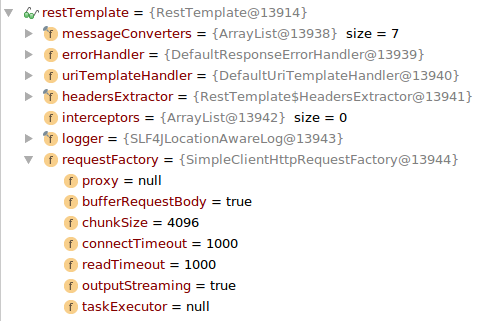
\includegraphics[scale=0.5]{resttempldatedefaulttimeout.png}
	\caption{RestTemplate默认超时时间}
	\label{fig:resttempldatedefaulttimeout}
\end{figure}

上图是Debug跟踪时查看的RestTemplate默认变量。由图中可以看出,默认超时时间是1秒。此时需要增大Read time out的默认超时时间。自定义Read time out超时时间如下代码片段所示:

\begin{lstlisting}[language=Java]
@Bean(name = "commonRestTemplate")
public RestTemplate restTemplate(RestTemplateBuilder restTemplateBuilder) {
	return restTemplateBuilder.setConnectTimeout(5000)
			.setReadTimeout(20000)
			.build();
}
\end{lstlisting}

出现此问题的原因是:当数据量较少时,请求基本能在非常短时间内响应,当数据量逐渐增加时,部分请求处理时间偶尔超过1秒,会出现偶尔失败的情况。

\subsection{自动化部署(Auto Deploy)}

\subsubsection{整体概况}

目前已经将自动化部署应用到部分项目中,省去了非常多手工操作。目前应用的项目情况一览表,表中,CI表示Continuous Integration。

\begin{table}[htbp]
	\caption{自动部署项目信息}
	\label{table:databaseconnectionpool}
	\begin{center}
		\begin{tabular}{|c|p{4.5cm}|p{4cm}|}
			\hline
			\multirow{1}{*}{项目名称}
			& \multicolumn{1}{c|}{中文名} 
			& \multicolumn{1}{c|}{说明}\\			
			\cline{1-3}
			report &  通用数据录入子系统  & 通过可灵活调整的配置,动态快速应对不同维度的数据录入场景 \\
			\hline
			report-frontend & 通用数据录入子系统(前端) & 通过可灵活调整的配置,动态快速应对不同维度的数据录入场景,提供动态渲染的,统一的UI \\
			\hline
			system & 主应用 & 主应用 \\
			\hline
			system-frontend & 主应用(前端) & 主应用(前端) \\
			\hline
			system-exchange & 数据交换(exchange)子系统 & 应对所有数据交换场景 \\
			\hline
			system-api & 接口(api)应用 & 接口应用,提供外部数据服务 \\
			\hline
			message & 消息系统 & 站内通知 \\
			\hline
			message-frontend & 消息系统(前端) & 站内通知 \\
			\hline
			web-ci & Web(Continuous Integration) & 网站 \\
			\hline
			web-ci-59 & Web & 网站 \\
			\hline
			web-ci-for-bid & Web & 网站(定制版) \\
			\hline				
		\end{tabular}	
	\end{center}
\end{table}

自动化部署服务器信息如表\ref{table:databaseconnectionpool}所示。提交代码后,构建服务器定时检查代码更新,检查周期可以通过cron表达式定义,若有变更,则触发自动编译构建。应用构建并打包完毕后,会通过调用文件中转服务,将编译完成的应用包拷贝到测试服务器指定目录下。测试服务器上会有定时任务定时调用Shell脚本,Shell脚本会监测应用文件的变化,或者版本定义文件中版本号的变化,任意一项有变动,则触发应用更新。版本变化通过读取版本配置文件来侦测,文件变化通过对比文件的Hash来判断。

\begin{table}[htbp]
	\caption{自动部署服务器信息}
	\label{table:databaseconnectionpool}
	\begin{center}
		\begin{tabular}{|c|c|p{5cm}|}
			\hline
			\multirow{1}{*}{IP}
			& \multicolumn{1}{c|}{名称} 
			& \multicolumn{1}{c|}{备注}\\			
			\cline{1-3}
			192.168.1.24 &  Jenkins服务器  & 所有项目的构建、编译、打包 \\
			\hline
			192.168.1.11 & Nginx服务器 & 文件的接收转发服务 \\
			\hline
			192.168.1.6 & App测试服务器 & 所有App运行在此服务器 \\
			\hline				
		\end{tabular}	
	\end{center}
\end{table}


\subsubsection{构建服务(Auto Build)}

构建服务包含获取源码更新、构建、构建后操作3步。由于项目针对不同应用场景,定义了不同的分支,所以在构建时,需要了解每个分支的含义。各分支定义如表\ref{table:projectbranch}所示:

\begin{table}[htbp]
	\caption{分支名称及含义}
	\label{table:projectbranch}
	\begin{center}
		\begin{tabular}{|c|c|p{6cm}|}
			\hline
			\multirow{1}{*}{项目名称}		 
			& \multicolumn{1}{c|}{分支名称}
			& \multicolumn{1}{c|}{备注}\\			
			\cline{1-3}
			system &  v1.3 & 主分支,1表示第几期,3表示阶段 \\
			\hline
			system & v1.3\_api & 接口分支 \\		
			\hline
			system & v1.3\_exchange & 数据交换分支 \\		
			\hline
			report & develop & 主分支 \\		
			\hline
			report-frontend & develop & 主分支 \\		
			\hline							
		\end{tabular}	
	\end{center}
\end{table}

构建服务定时检查源码仓库的变动,监测到变动后,触发自动编译打包等操作。构建后,通过调用构建后脚本,将文件拷贝到服务器。构建后脚本路径/home/jenkins-bak/,各个脚本的含义如表\ref{table:handlernamingrule}日所示。

\begin{table}[htbp]
	\caption{自动部署后触发脚本命名规则}
	\label{table:handlernamingrule}
	\begin{center}
		\begin{tabular}{|p{7cm}|p{3.5cm}|}
			\hline
			\multirow{1}{*}{脚本名称}		 
			& \multicolumn{1}{c|}{备注}\\			
			\cline{1-2}
			\{prject-name\}-after-build-handler.sh &  项目后端构建后处理 \\
			\hline
			\{project-name\}-frontend-after-build-handler.sh  & 项目后端构建后处理 \\		
			\hline				
		\end{tabular}	
	\end{center}
\end{table}

脚本命名含义一般是项目名称加需要产生的作用,project-name表示对应的项目名字,新增时可替换为项目的实际名称。after-build-handler表示此脚本主要告诉Jenkins构建后需要执行此脚本完成一系列动作。构建需要特殊处理的地方:


\begin{lstlisting}[language=Bash]
#!/usr/bin/env bash

# 当使用未初始化的变量时,程序自动退出
set -u

# 当任何一行命令执行失败时,自动退出脚本
set -e

# 在运行结果之前,先输出执行的那一行命令
set -x

readonly APP_ID=""
readonly APP_KEY=""
readonly PROJECT_DIR="/var/lib/jenkins/workspace/web-ci-59"
readonly BUILD_OUTPUT_DIR="/var/lib/jenkins/workspace/web-ci-59/cms/target"

BUILD_DIST_FILENAME=${BUILD_OUTPUT_DIR}/cms.war

cd ${BUILD_OUTPUT_DIR}

#
# 文件过大,无法拷贝
# 将大文件拆分
#
split -b 80M ${BUILD_DIST_FILENAME}

CURRENT_TIME=`date '+%Y-%m-%d %H:%M:%S'`

CONST_STR="ysf"

#
# 生成TOKEN
# 接口各项认证参数的排列顺序是:
# 时间戳(timestamp)、AppKey、随机字符串(echostr)
#
TOKEN=`echo -n ${APP_ID}${APP_KEY}${CURRENT_TIME}${CONST_STR}|md5sum|awk '{print $1}'`
SEQUENCE_TOKEN=`echo -n ${CURRENT_TIME}${APP_ID}${APP_KEY}${CONST_STR}|shasum -a 1|awk '{print $1}'`


# 请求服务端,上传主文件
COMMAND=`curl -H "APPID:$APP_ID" \
-H "TIMESTAMP:$CURRENT_TIME" \
-H "ECHOSTR:$CONST_STR" \
-H "TOKEN:$SEQUENCE_TOKEN" \
-F "file=@${BUILD_OUTPUT_DIR}/xaa" \
http://192.168.1.11:8083/api/fileExchange/upload`

COMMAND=`curl -H "APPID:$APP_ID" \
-H "TIMESTAMP:$CURRENT_TIME" \
-H "ECHOSTR:$CONST_STR" \
-H "TOKEN:$SEQUENCE_TOKEN" \
-F "file=@${BUILD_OUTPUT_DIR}/xab" \
http://192.168.1.11:8083/api/fileExchange/upload`
\end{lstlisting}

在上传文件时,由于限制了文件大小(估计是100MB),当部署文件大于100MB时,使用split命令,拆分成多个小文件分开上传,上传后通过cat命令组装成war包,组装后的文件与原始文件一致,可以通过对比文件的MD5值来判断。

\subsubsection{中转服务(Forward Service)}

中转服务将构建服务器上生成的应用包转发到应用服务器,应用包在测试服务器192.168.1.6的存放路径是/home/deploy/credit。中转服务的配置主要是Nginx转发上传的请求到指定服务器:

\begin{lstlisting}[language=Bash]
location /api/fileExchange {
	proxy_pass http:ip:port;
	proxy_redirect off;
}
\end{lstlisting}

\subsubsection{应用更新服务(Update Trigger)}

应用更新服务在测试服务器,通过建立cron定时任务,轮询检查应用更新情况。定时任务配置文件是/etc/crontab,各个系统更新触发脚本路径是/opt/app/script。定时任务配置示例:

\begin{lstlisting}[language=Bash]
#
# project name update trigger
#
*/1 * * * * root /opt/app/script/project-name-trigger.sh
\end{lstlisting}

触发更新规则在相应的Shell脚本中实现。如下代码片段所示:

\begin{lstlisting}[language=Bash]
#!/usr/bin/env bash

# 部署触发器
# 定时检查文件修改
# 文件修改后,触发部署动作

# 当使用未初始化的变量时,程序自动退出
#set -u

# 当任何一行命令执行失败时,自动退出脚本
set -e

# 在运行结果之前,先输出执行的那一行命令
set -x

# 定义错误日志级别
LOG_LEVEL=-9000

#定义日志存放目录
SIMPLE_LOG_4_SH_DIR=/tmp/simplelog4sh

#导入日志
. /opt/app/script/log4shell.sh

# 当前运行程序版本
readonly APP_PATH="/opt/app/backend-v1.3"
readonly DEPLOY_PATH="/home/deploy/credit"
source ${APP_PATH}/report-version.properties
CURRENT_VERSION=${VERSION}
source ${DEPLOY_PATH}/report-version.properties
DEPLOY_VERSION=${VERSION}
readonly FILE_NAME="report-web-boot-${CURRENT_VERSION}.jar"
readonly DEPLOY_FILE_NAME="report-web-boot-${DEPLOY_VERSION}.jar"

logInfo "检查后端App更新..."

deploy()
{
	logInfo "停止旧版本程序...,版本:${CURRENT_VERSION}"
	ps -ef|grep -w ${FILE_NAME}|grep -v grep|cut -c 9-15|xargs kill 9
	logDebug "开始拷贝新版程序文件....."
	yes|cp -rf ${DEPLOY_PATH}/${DEPLOY_FILE_NAME} ${APP_PATH}
	yes|cp -rf ${DEPLOY_PATH}/credit-report-version.properties ${APP_PATH}
	logInfo "启动新版程序......,程序路径:${APP_PATH},版本:${DEPLOY_VERSION}"
	${APP_PATH}/start-v1.3.sh
}

if test ${CURRENT_VERSION} = ${DEPLOY_VERSION}
then
	logInfo "版本号无变化,检查文件Hash...."
	CURRENT_VERSION_MD5=`md5sum ${APP_PATH}/${FILE_NAME}|cut -d ' ' -f1`
	DEPLOY_VERSION_MD5=`md5sum ${DEPLOY_PATH}/${FILE_NAME}|cut -d ' ' -f1`
	if test ${CURRENT_VERSION_MD5} != ${DEPLOY_VERSION_MD5}
	then
		deploy ""
	else
		logInfo "Hash无变化,文件未修改,后端App结束..."
	fi
else
	logInfo "后端App版本有变化,开始部署新版程序..."
	deploy ""
fi
\end{lstlisting}

由于目前应用较多,单独列出每个应用的目录比较冗长。此处仅仅描述目录的命名的一般性原则。测试环境的目录统一在opt下(项目初始阶段习惯),正式环境的目录在根目录home(初始习惯)或者data下,data目录存放应用是推荐的标准做法,以后新应用部署推荐用此标准,data下存放组织名称对应的目录,组织名称下对应此组织相应的应用。当前各个应用的目录如表\ref{table:projectdirectionayinfo}所示。recommand表示推荐做法,obsolete表示过时的做法,以后不推荐采用的方式。Test表示测试环境,对应的测试服务器IP,Production表示生产环境,对应的生产环境的IP。

\begin{table}[htbp]
	\caption{项目部署目录信息}
	\label{table:projectdirectionayinfo}
	\begin{center}
		\begin{tabular}{|c|p{4cm}|p{4cm}|}
			\hline
			\multirow{1}{*}{环境}
			& \multicolumn{1}{c|}{目录}
			& \multicolumn{1}{c|}{备注}\\			
			\cline{1-3}
			Test  & /opt/app/ & 部署目录 \\
			\hline
			Test  & /home/deploy/credit/ & CI部署文件存放目录 \\
			\hline
			Test  & /opt/app/script/ & CI部署脚本存放目录 \\
			\hline
			Prod  & /home/app/ & \textcolor{red}{obsolete} \\
			\hline
			Prod  & /data/\{companyname\}/app/ & \textcolor{green}{recommand} \\
			\hline							
		\end{tabular}	
	\end{center}
\end{table}

\subsection{Nginx超时转发}

在后端有双机或多台机器提供服务的情况下,如果某一台机器超过了一定时间未响应,Nginx将尝试将请求转发到下一台服务器。由于写操作时,如果没有在后端作重复校验,一旦写操作比较耗时,转发后会出现重复写的情况(POST一般不进行超时转发,但是幂等请求下也可能会产生重复,比如日志记录、触发消息通知等等)。避免此问题的一种设计方案是在前端渲染表单时,生成一个唯一ID,防止重复提交。所以此处仅仅将超时转发的规则应用在部分url上,在Nginx中的配置如下:

\begin{lstlisting}[language=Bash]
upstream example_upstream{
	server 192.168.0.1 max_fails=1 fail_timeout=3s;
	server 192.168.0.2 max_fails=1 fail_timeout=3s backup;
}
location /example/ {
	proxy_pass http://example_upstream/;
	proxy_set_header Host: test.example.com;
	proxy_set_head X-real-ip $remote_addr;
	proxy_next_upstream error timeout http_500;
}
\end{lstlisting}

Nginx在POST, LOCK, PATCH这种会对服务器造成不幂等的方法,默认是不进行重试的,如果一定要进行重试,则要加上如下配置:

\begin{lstlisting}[language=Bash]
# 非幂等也进行超时转发配置
proxy_next_upstream error timeout http_500 non_idemponent;
\end{lstlisting}




\subsection{无法获取数据库连接}

\begin{quote}
	\textbf{\textcolor{red}{导致问题的原因:数据库连接配置过小,访问量增长时造成连接分配不足,导致无法顺畅访问站点。}}
\end{quote}

最近2天网站运行一段时间后会突然宕掉,日志输出无法获取数据库连接(Could not get JDBC connection),初步推测是数据库连接泄漏,造成数据库可用连接被使用完,主备节点都拿不到连接,造成此问题,目前连接由连接池进行管理,一般情况下是不需要人工干预数据库的连接申请和释放,也有可能是某处进行了手工申请数据库连接,但是没有释放连接导致。使用如下Shell脚本每隔一段时间检测连接池数量:

\begin{lstlisting}[language=Bash]
# 每5秒查看一次到数据库连接个数
nohup watch -n 5 'lsof -i:5236|wc -l >> pool.log'
\end{lstlisting}

经过观察,数据库连接稳定在300-310之间,如果是连接池泄漏,那么连接会随着程序运行逐渐增长,最终达到连接数量上限,根据观察,初步可以排除连接泄漏导致此问题。后来经过日志筛查,发现如下输出:

\begin{lstlisting}[language=Bash]
# 活动连接数
active 20,maxActive 20
\end{lstlisting}

表示当前活动连接数20个,最大活动连接数20个。虽然到数据库的会话有300多个,但是绝大多数是空闲的(Idle),如下语句查看数据库当前会话的个数。

\begin{lstlisting}[language=SQL]
-- 查看数据库当前会话情况
select clnt_ip,state,user_name,count(*)
from v$sessions
group by clnt_ip,state,user_name
\end{lstlisting}

结果如图\ref{fig:sessionstatistics}所示:

\begin{figure}[htbp]
	\centering
	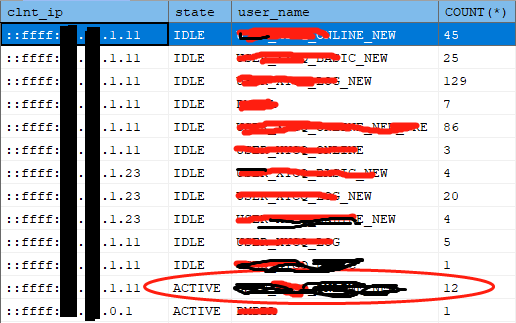
\includegraphics[scale=0.6]{sessionstatistics.png}
	\caption{DB当前连接会话统计}
	\label{fig:sessionstatistics}
\end{figure}

可以看出,活动的会话稳定在13个,离最大个数20已经不远,极有可能是数据库会话配置过小,导致用户增多时,无可用连接分配。为了验证推断,使用JMeter\footnote{\url{http://jmeter.apache.org/}}模拟多用户同时访问测试网站。逐步增加同时访问的用户的个数,当增加到80个时,网站无响应。检查后端日志,出现了线上的问题同样的日志输出,说明问题在此处,需要优化。DBCP当连接数超过最大连接数时,所有连接都会被断开[未找到权威出处]。经过考虑,逐步应用以下优化的方式。

\paragraph{增加网站数据库连接数量上限}调整配置增大数据库连接上限,可以增加网站并发服务能力:

\begin{lstlisting}[language=XML]
<!-- 最小空闲连接数 -->
<property name="minIdle" value="50" />
<!-- 最大连接数 -->
<property name="maxActive" value="100" />
\end{lstlisting}

做了以上优化后,可以提高网站的并发服务量,降低由于访问量过大造成网站不可用的概率,20个连接确实太小,综合评估数据库现有的连接资源(500),调整后连接数分配情况:

\begin{table}[htbp]
	\caption{应用连接个数分配情况}
	\label{table:projectdirectionayinfo}
	\begin{center}
		\begin{tabular}{|p{3cm}|c|p{2cm}|}
			\hline
			\multirow{1}{*}{环境}
			& \multicolumn{1}{c|}{IP} 
			& \multicolumn{1}{c|}{连接个数}\\			
			\cline{1-3}
			主机 &  192.168.1.1  & 100 \\
			\hline
			备机 &  192.168.1.23  & 100 \\
			\hline
			移动端 &  192.168.1.1  & 100 \\
			\hline
			旧版App、定制版App、登陆、临时使用预留 &  192.168.1.*  & 200 \\
			\hline									
		\end{tabular}	
	\end{center}
\end{table}

增加了连接数上限后,为了验证效果,采用crontab定时任务每隔5分钟定时采集不同时间点数据库的活动Session个数:

\begin{lstlisting}[language=Bash]
# 每5分钟定时执行采集任务
*/5 *  *  *  *  root   /usr/local/dolphin/script/db-pool-monitor.sh
\end{lstlisting}

脚本将采集到的数据放入csv文件中,后期采用Excel生成可直观的图表:

\begin{lstlisting}[language=Bash]
#!/usr/bin/env bash

# 当使用未初始化的变量时,程序自动退出
set -u

# 当任何一行命令执行失败时,自动退出脚本
set -e

# 在运行结果之前,先输出执行的那一行命令
set -x

connect_size=`lsof -i|grep 10.20.1.17|grep java|wc -l`
current_time=`date "+%H:%M:%S"`
current_date=`date "+%Y%m%d"`
echo "${current_time},${connect_size}" >> /home/monitor/dm-pool-"${current_date}".csv
\end{lstlisting}

数据库实时Session监控脚本向csv中写入2列,当前的时间和当前时间点的活动Session的个数,每天生成一个csv文件。根据csv生成的折线图效果如图\ref{fig:dbsession}所示。

\begin{figure}[htbp]
	\centering
	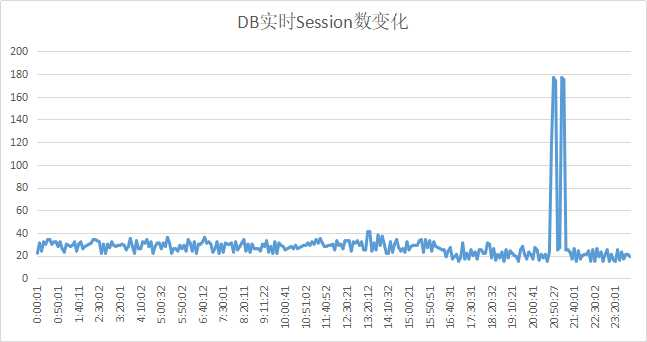
\includegraphics[scale=0.5]{dbsession.bmp}
	\caption{DB历史会话数统计}
	\label{fig:dbsession}
\end{figure}


8:50到9:40时间段进行了压力测试,这个时间范围内数据库的活动Session有明显的增加。

\paragraph{增大数据库Session数量上限}目前数据库的会话数量是500,可以调整为1000。

\paragraph{缓存页面信息}实际上,页面在绝大部分时间是不会改变的,完全可以将页面信息缓存在Redis中,不但减轻数据库压力,还可成倍提高网站响应速度和并发处理能力。此种优化方式需要对代码做一定程度改造,比如发布信息时,需要清除对应模块的Redis缓存信息,保证信息更新及时。

\paragraph{将流量分配到不同的机器}后端流量可以主备机同时启用,涉及到Session共享问题,需要进一步测试。




\subsection{Java heap space}

\begin{quote}
	\textbf{\textcolor{red}{导致问题的原因:表面看是APP分配的内存资源不足,系统并发性能不足,应对持续并发请求能力需要加强,实际是Tomcat请求头配置过大(100MB),每个线程会申请对应大小的空间,而大对象JVM直接会放到老年代,一旦并发请求稍多,造成内存溢出。}}
\end{quote}

上周网站Down掉,本周接口Down掉,愉快的周末泡汤了。所以,暗自忖度,一定要找到问所在。Heap的大小是Young Generation 和Tenured Generaion 之和。在JVM中如果98\%的时间是用于GC,且可用的Heap size 不足2\%的时候将抛出此异常信息。内存溢出一般分为2种情况,一时是超出预期的访问量/数据量,另一种是内存泄露(Memory leak)。第一次的内存溢出异常有hprof文件,将文件拷贝出来进行分析。第二次接口异常没有生成hprof,采用VisualVM\footnote{VisualVM在JDK安装包中附带,在\$JAVA\_HOME/bin目录下。}分析内存情况。新建

\begin{lstlisting}[language=Bash]
grant codebase "file:/home/local/jdk1.8.0_111/lib/tools.jar" {   
	permission java.security.AllPermission;   
};
\end{lstlisting}

在服务端启动jstatd(Java State Daemon)守护进程:

\begin{lstlisting}[language=Bash]
# 启动统计守护进程
./jstatd -J-Djava.security.policy=../jstatd.all.policy -J-Djava.rmi.server.hostname=10.10.1.53
# 生成内存dump文件
jmap -dump:format=b,file=/opt/example.dump [pid]
\end{lstlisting}

在本地使用VisualVM监视服务端JVM的运行情况,内存的增长速度在4-5MB/s,2GB的内存在4-5min就被消耗完毕,接着进行一次YGC(Young Garbage Collection)。初步监测,老年代(Old Generation)的内存的确在不断增长。但是仅凭此点,无法下结论一定存在内存泄漏,如果老年代在以后执行GC(Garbage Collection)后,老年代(Old Generation)初始内存不停增长,才可以推断的确存在内存泄漏,因为不停增加的初始内存,标志着有部分内存永远无法被FGC回收,随着程序的不断运行,必定会由于内存不足而Hang住。

\begin{table}[htbp]
	\caption{应用内存消耗}
	\label{table:appmemoryusing}
	\begin{center}
		\begin{tabular}{|c|c|p{2cm}|}
			\hline
			\multirow{1}{*}{并发数量}
			& \multicolumn{1}{c|}{Old Generation内存消耗} 
			& \multicolumn{1}{c|}{连接个数}\\			
			\cline{1-3}
			0 &  404MB  & 100 \\
			\hline
			1 &  1.119GB  & 100 \\
			\hline
			10 &  3.847GB  & 100 \\
			\hline
			20 &  3.689GB  & 100 \\
			\hline
			30 &  4.834GB  & 100 \\
			\hline											
		\end{tabular}	
	\end{center}
\end{table}

在一段时期内,程序一启动老年代就已经满了,占用率直接100\%。开始是以为流量较高,YGC频繁,不停的有经过多次YGC未回收的对象移入老年代,最多FGC执行频繁一些罢了。后来更为诡异的事情发生了,机器突然变得非常卡顿,磁盘使用量快速增长,最后程序直接无法启动,启动不到30s立即停止响应或者直接输出Java Heap space错误。

\paragraph{问题复现}

经过备份的日志阅读,发现一段时间段内,有大量针对某一查询请求,且非常集中。下午抽出时间在测试环境使用JMeter构造红集中请求的查询,模拟线上场景。当并发的用户量不断增长时,YGC越来越频繁,同时老年代初始内存消耗上升快速。当并发量达到50时,老年代内存使用量飙升到100\%,同时程序Hang住,输出Java Heap space错误。终于知道症结在机器在应对并发流量时内存不足,没有对内存做好估算。并发量升高时,应用对的内存消耗极大的超出了预期,即使每个线程5MB的内存,100个并发也才500MB,当前的内存有5GB,按照预期是完全足够的。但最终还是将服务器的内存增大到64GB来解决问题。

\paragraph{问题回顾}

当在并发量较高时,APP启动时,会占用比较多的老年代内存,所以在下午应用已启动老年代内存立即耗尽,年轻代不停的执行GC。当并发超出系统承载能力时,老年代默认内存已经无法支撑应用启动的初始内存消耗,所以应用启动立即发生内存溢出。有于在发生内存溢出时会生成dump文件,将现场保留到磁盘以备问题排查,每个dump文件从2GB-8GB不等,所以造成磁盘使用量急速消耗。

\begin{lstlisting}[language=Bash]
# 内存溢出时生成dump文件
-XX:+HeapDumpOnOutOfMemoryError 
-XX:HeapDumpPath=/home/app
\end{lstlisting}

不停的尝试启动,不停的生成dump文件,造成磁盘IO急剧升高,所以机器卡顿。

\paragraph{问题解决}

一是增大系统并发吞吐量,二是系统需要有限流和熔断机制。为了避免类似情况,系统做如下优化:

\begin{itemize}
	\item {一是将热点查询做成静态化页面,针对一级页面,打开即默认加载的数据静态化,避免后端接口处理,降低接口压力。}
	\item {二是缓存凭据,凭据信息更改不频繁,直接缓存到内存中,避免数据库查询。}
	\item {三是评估内存消耗,针对设计预期的并发分配相应的资源。}
	\item{四是限流,识别无效请求并主动丢弃,减少无效流量对资源的占用和消耗,可以根据实时流量调整限制级别。例如在平时网站运行时,可以将限制关闭,在应对重大事件时,可以将限制开启并根据网站保障级别调整限制级别。}
	\item {五是使用监控工具,对网站的实时流量和服务器负载有监控预警,根据流量情况采取不同的措施。}
\end{itemize}

关键的问题是,在当前并发的情况下,不应该消耗如此大的内存。问题在哪里?使用JMap\footnote{\url{https://docs.oracle.com/javase/7/docs/technotes/tools/share/jmap.html}}(Java Memory Map)命令将运行时内存情况输出,采用MAT\footnote{\url{https://www.eclipse.org/mat/}}(The Eclipse Memory Analyzer)工具进行分析,查看内存中的大对象如图\ref{fig:javahprofanalysis}所示。

\begin{figure}[htbp]
	\centering
	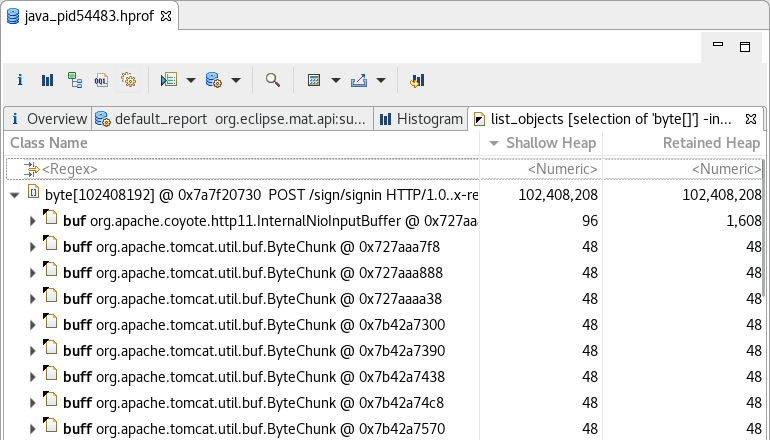
\includegraphics[scale=0.3]{javahprofanalysis.png}
	\caption{Java内存对象分析}
	\label{fig:javahprofanalysis}
\end{figure}

从Histogram图中可以看出,对象中byte数组的大小超过了8GB,每一个byte数组元素大小是102408208(约102MB)。怎么会有如此大对象?问题非常有可能就出在这些大对象上面了。下载Tomcat 8.0.53(注意下载的源码需要尽量服务器上运行的版本一致,InternalNioInputBuffer类在往后版本的Tomcat已经被移除)源码查看,找到如下代码片段:

\begin{lstlisting}[language=Java]
@Override
protected void init(SocketWrapper<NioChannel> socketWrapper,
AbstractEndpoint<NioChannel> endpoint) throws IOException {

	socket = socketWrapper.getSocket();
	if (socket == null) {
		// Socket has been closed 
		// in another thread
		throw new IOException(sm.getString("iib.socketClosed"));
	}
	socketReadBufferSize =
	socket.getBufHandler().getReadBuffer().capacity();
	
	int bufLength = headerBufferSize + socketReadBufferSize;
	if (buf == null || buf.length < bufLength) {
		buf = new byte[bufLength];
	}
	
	pool = ((NioEndpoint)endpoint).getSelectorPool();
}
\end{lstlisting}

在处理请求的线程初始化时,根据请求头大小新构建一个byte数组(\textcolor{red}{new byte[bufLength]}),原来是请求头设置过大。系统在生成byte数组时,判断是大对象,直接将对象放到老年代中,造成老年代消耗内存急速增长。

\subsection{报表在现场演示环境无法打开}

\begin{quote}
	\textbf{\textcolor{red}{导致问题的原因:报表地址配置的内网地址,公网用户无法访问。}}
\end{quote}

报表服务部署在内网的机器上,内网的机器与平时使用的机器在一个局域网中,内网用户访问报表可以直接通过内网IP。但是公网的用户无法访问报表服务器的内网IP,需要通过公网IP做一次转发。就像在自己家里部署一个服务,但是在办公室的PC是无法访问的,需要有公网IP做转发。公网用户访问报表的一般流程是,先访问公网地址,公网地址将流量转发到内网的反向代理服务器,反向代理服务器根据报表的URL将流量路由到报表服务器。使用如下语句更新报表配置即可:

\begin{lstlisting}[language=SQL]
# 将报表服务的IP调整为公网IP
update report_config
set url = replace(url,'内网IP','公网IP')
\end{lstlisting}

\subsection{查询变慢}

\begin{quote}
	\textbf{\textcolor{red}{导致问题的原因:日志数据不断膨胀造成查询变慢,日志记录的方式需要优化。}}
\end{quote}

这两天不断有反馈原来很快的查询现在不知道什么原因变慢了,查看了变慢的页面后,确实速度不符合设计预期,正常情况下不应大于200ms,平均响应时间肯定不会超过1s,页面数据是放在接口缓存中。加上调用链路的开销,不应该有延迟。访问接口数据的流程如图\ref{fig:api-request}所示:

\begin{figure}[htbp]
	\centering
	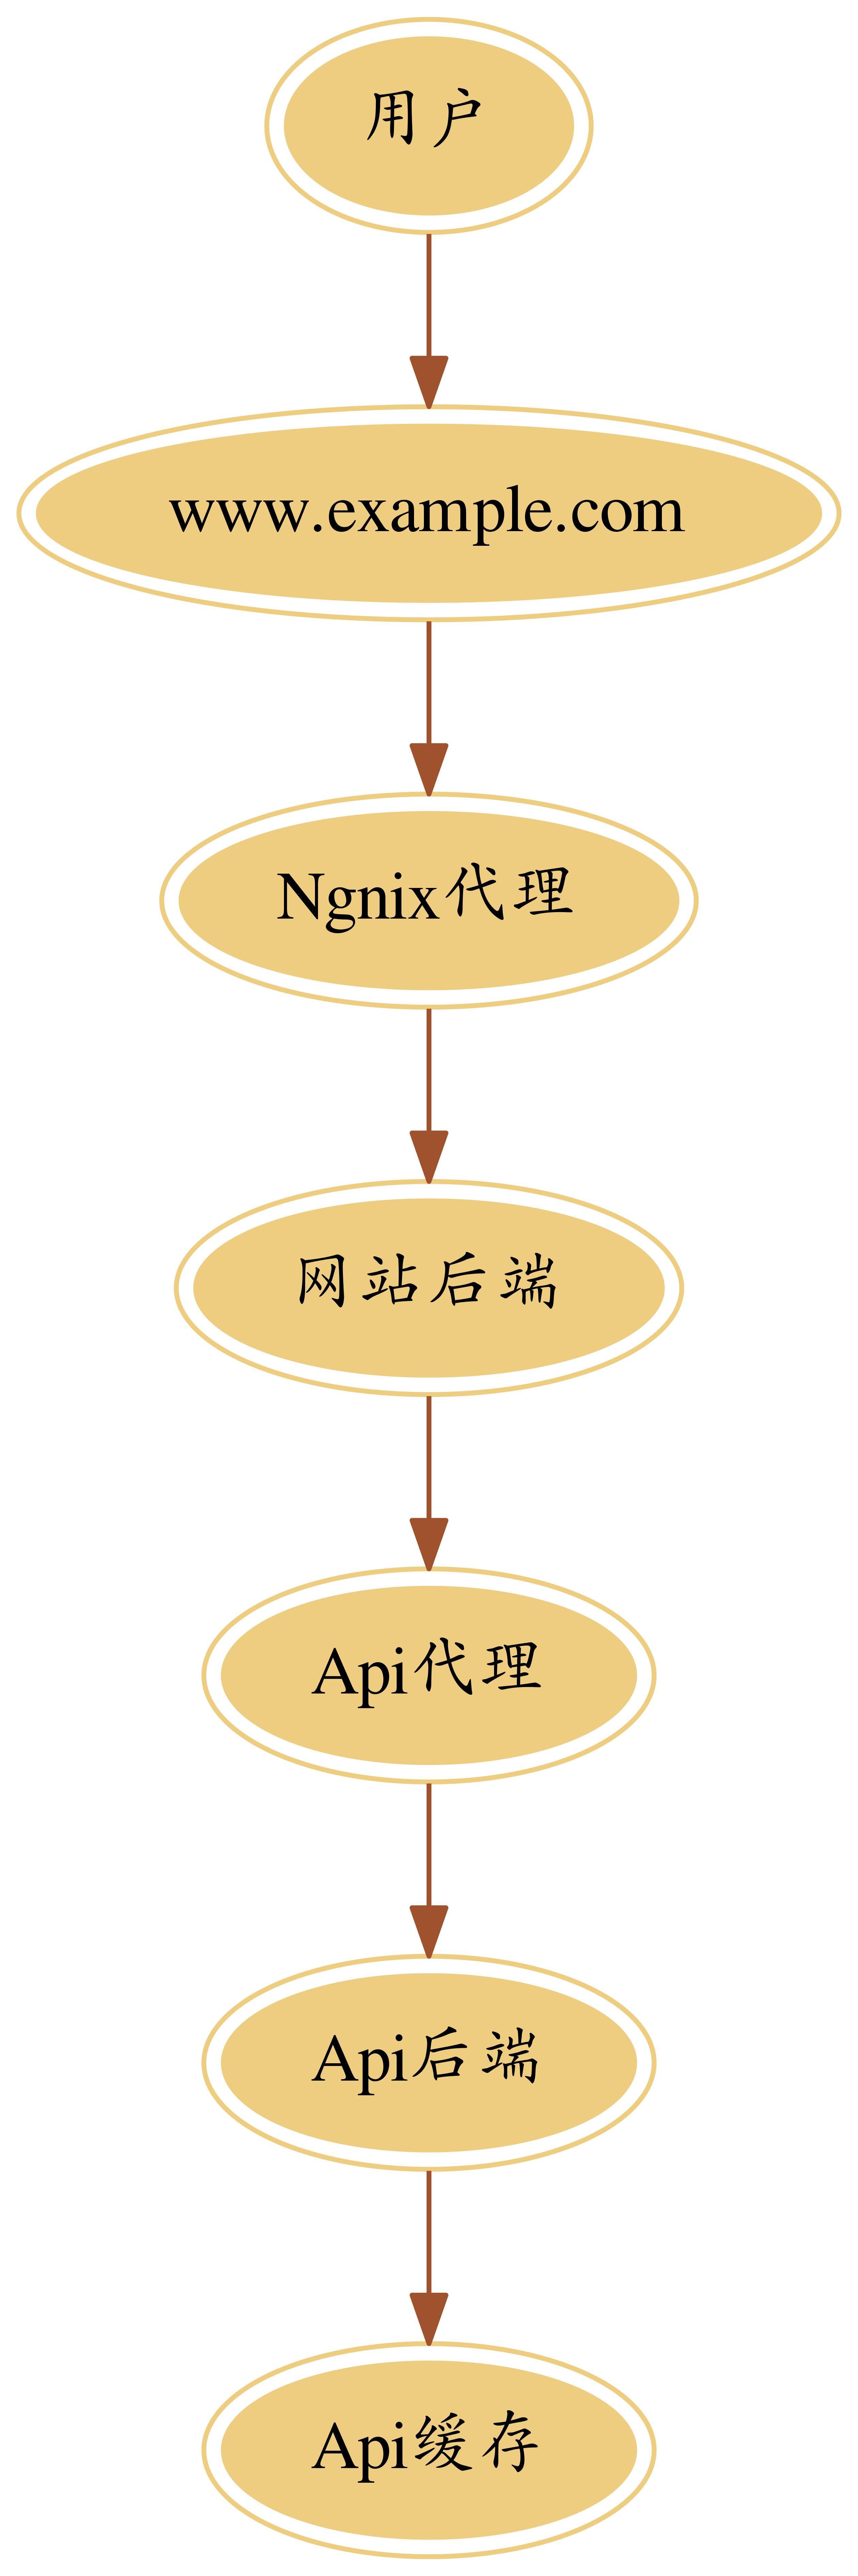
\includegraphics[scale=0.08]{api-request.jpg}
	\caption{接口数据调用流程}
	\label{fig:api-request}
\end{figure}

首先确定接口缓存有效,在接口服务器上请求接口服务:

\begin{lstlisting}[language=Bash]
curl -H "APPID:" \ 
-H "TIMESTAMP:2016-12-19 16 (tel:2016121916):58:02" \ 
-H "ECHOSTR:sdsaasf" -H "TOKEN:" \
-H "Accept: application/json, text/plain" \ 
http://192.168.1.11:28081/api/example?name=\&page=1\&size=10|jq '.'
\end{lstlisting}

在50ms内可以返回结果,说明缓存有效,不是从数据库获取。其次确定网络设备影响(已经感受到的发送POST请求会有1-2s左右延迟,网络A的服务器发出请求,网络B的服务器需要1-2s才能实际接收到并处理),在网络A使用访问接口服务,时间与网络B访问相近。由于端口80绑定域名,新建内网服务,从内网站点访问接口,时间超过3s,说明问题在A网的站点。后经过跟踪,发现A网站点接口本身处理非常快,但是绝大部分时间消耗在处理请求后返回的过程中。经过跟踪,处理请求后查询更新了日志表,而日志表的数据在800W左右。

\paragraph{问题解决}

\begin{itemize}
	\item {快速的解决方式,临时备份日志,建立空的日志表。}
	\item {重构日志,直接记录流水,不记录统计信息。(\textcolor{green}{\textbf{Recommand}})}
	\item {构建独立的日志服务,所有的日志打到独立的服务上,采用简单消息队列。(\textcolor{green}{\textbf{Recommand}})}
	\item {尝试ELK日志分析系统。}
\end{itemize}

\subsection{资源分配约定}

由于最近处理的问题大多涉及到资源问题,例如文件无法上传,邮件无法发送,主要由于磁盘空间不足。原来分配的虚拟机一般home目录较大,所以将随着程序运行可能需要消耗较大磁盘空间的目录放在home目录下,但是新内网虚拟机恰好home目录很小。导致一些列问题,所以这里约定新部署App目录的统一规范。

\begin{table}[htbp]
	\caption{磁盘目录分配约定}
	\label{table:}
	\begin{center}
		\begin{tabular}{|c|p{5cm}|}
			\hline
			\multirow{1}{*}{路径}
			& \multicolumn{1}{c|}{用途}\\			
			\cline{1-2}
			/opt/alibaba/app &  存放项目应用程序  \\
			\hline
			/opt/alibaba/var/data & 存放数据文件 \\
			\hline			
			/opt/alibaba/var/image & 存放图片文件 \\
			\hline
			/opt/alibaba/local & 存放三方程序 \\
			\hline
			/opt/alibaba/backup & 存放备份文件 \\
			\hline
			/opt/alibaba/logs & 存放日志文件 \\
			\hline														
		\end{tabular}	
	\end{center}
\end{table}

考虑到安全,程序启动须使用alibaba帐号,不使用root启动应用程序。日志应独立存放,避免放到应用目录下,因为日志文件通常会比较大,独立存放日志好处之一是在新应用部署时,可以直接拷贝app目录,而避免与日志一起拷贝或者需要单独做一步忽略日志的操作。




\subsection{Tomcat请求头设置}

App在启动的时候占用老年代内存较大,当并发增大时,消耗内存迅速增加。经过排查,是maxHttpHeaderSize参数配置过大。

\begin{lstlisting}[language=Bash]
#
# 请求头允许的最大长度,单位为KB
# 如果没有指定,默认是8192(8KB)
# 这里请适当斟酌,在批量查询时
# URI中需要带参数(批量查询的参数会比较大)
# 点击返回按钮后
# 需要根据URI中记录的参数定位到上一个页面
# 如果不增加Header Size
# 没有更好的方案实现返回功能
# 所以Header Size设置得较大
#
server.max-http-header-size=102400000
\end{lstlisting}

这种问题应该是很明显的,为何到现在才发现?对比了旧版的配置,旧版配置的是1MB。估计在新版配置的时候顺手将开发环境的配置拷贝到生产,而开发环境的配置比较随意。Tomcat在处理HTTP请求时,会直接申请maxHttpHeaderSize大小的内存空间,而不仅仅是一个限制。


\subsection{GoAccess}

最近网站流量“偏高”,导致关键服务停服。所以可以考虑实时的监控网站的健康状态,作出对应的决策。由于安全原因不能使用监控应用,所以找到一个直接在终端下可以查看Nginx日志统计信息的应用GoAccess\footnote{\url{https://goaccess.io}}。

\begin{lstlisting}[language=Bash]
goaccess -a -d -f /usr/local/nginx/logs/example.log
goaccess -a -d -f /usr/local/nginx/logs/example.log -p /etc/goaccess.conf -o /data/html/hexo/public/go-access.html
\end{lstlisting}

不能以服务的方式运行,所以做一个crontab定时任务,每隔一段时间生成网站访问日志的统计信息:

\begin{lstlisting}[language=Bash]
# 每20分钟执行
*/20 * * * *   root   goaccess -d -f /usr/loca/nginx/logs/example.log -p /usr/local/etc/goaccess.conf
\end{lstlisting}

根据URL的访问频率统计信息如图\ref{fig:spideranalysis}所示,从统计图中可以看出,九成以上的请求都集中在一个URL。



根据IP的统计信息如图\ref{fig:ipstatistics}所示,从统计图中可以看出,5成以上的访问请求只服务了3个IP。



\subsection{Nginx启用压缩}

最近演示时说系统很慢,打开系统查看,首屏加载时间超过8s,确实不符合常规。由于网站是SPA应用,首先查看Javascript大小,竟然有接近8MB大小,对比了线上系统,发现演示系统Javascript没有压缩。这里经过了两级Ngnix代理,内网访问Ngnix代理,浏览器中查看Javascript大小在1.6MB左右,说明内网的Nginx代理已经压缩了Javascript文件,推测可能是另一级需要对代理Nginx做启用gzip压缩配置,尝试在另一级Nginx代理添加如下配置:

\begin{lstlisting}[language=Bash]
# HTTP代理版本(proxy\_http\_version)
proxy_http_version 1.1
# gzip支持版本(gzip\_http\_version)
gzip_http_version 1.0
\end{lstlisting}

gzip模块默认支持压缩的HTTP版本是1.1,而代理模块的默认代理HTTP版本是1.0\footnote{\url{https://reinout.vanrees.org/weblog/2015/11/19/nginx-proxy-gzip.html}},不匹配,造成gzip的压缩没有生效,调整任意一项即可。

\subsection{查看网站并发}

使用如下命令查看网站并发:

\begin{lstlisting}[language=Bash]
netstat -n | awk '/^tcp/ {++S[$NF]} END {for(a in S) print a, S[a]}'

# 查看Ngni并发
tail -f access.log | awk -F '[' '{print $2}' | awk 'BEGIN{key="";count=0}{if(key==$1){count++}else{printf("%s\t%d\r\n", key, count);count=1;key=$1}}'
\end{lstlisting}

结果如图\ref{fig:websiteconcurrentaccess}所示:



\begin{lstlisting}[language=Bash]
goaccess -a -d -f /data/logs/fanhaobai.com.access.log -p /etc/goaccess.conf -o /data/html/hexo/public/go-access.html
\end{lstlisting}

不能以服务的方式运行,所以做一个crontab定时任务,每隔一段时间生成网站访问日志的统计信息:

\begin{lstlisting}[language=Bash]
# 每20分钟执行
*/20 * * * *   root   goaccess -d -f /usr/loca/nginx/logs/example.log -p /usr/local/etc/goaccess.conf
\end{lstlisting}

根据URL的访问频率统计信息如图\ref{fig:spideranalysis}所示,从统计图中可以看出,九成以上的请求都集中在一个URL。

\begin{figure}[htbp]
	\centering
	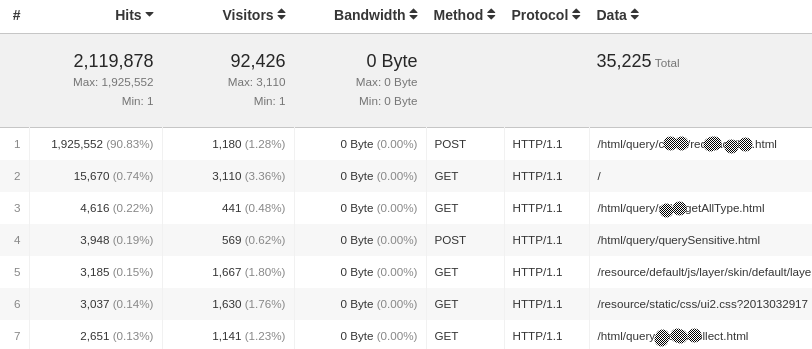
\includegraphics[scale=0.35]{spideranalysis.png}
	\caption{访问URL统计}
	\label{fig:spideranalysis}
\end{figure}


根据IP的统计信息如图\ref{fig:ipstatistics}所示,从统计图中可以看出,5成以上的访问请求只服务了3个IP。



\subsection{自动构建更新的问题}

有时经常会遇到代码提交后在测试环境总看不到效果的问题。可以使用如下方式逐步排查。第一步检查Jenkins是否获取到了最新的代码,在Jenkins构建目录(/var/lib/jenkins/workspace)下检查最新代码片段。第二步检查Tomcat目录下是否包含最新的调整后的代码,由于Tomcat下是已经编译完毕的class文件,需要借助Luyten\footnote{Luyten是一个出色的Java反编译器,项目地址是\url{https://github.com/deathmarine/Luyten}。}工具打开,查看源码,是否包含最新的改动,如果包含最新改动,说明自动编译构建没问题。这里查看Tomcat下的class文件包含了最新的调整,但是没有自动更新,重启Tomcat后更新生效。尝试调整发布脚本,每次发布时重新启动Tomcat来解决此问题。

\begin{lstlisting}[language=Bash]
#!/usr/bin/env bash

# 当使用未初始化的变量时,程序自动退出
set -u

# 当任何一行命令执行失败时,自动退出脚本
set -e

# 在运行结果之前,先输出执行的那一行命令
set -x

readonly AUTO_BUILD_OUTPUT_PATH="/var/lib/jenkins/workspace/dolphin/api/target"
readonly PROGRAM_NAME="cms.war"
readonly DEPOLY_PATH="/opt/alibaba/local/apache-tomcat-8.0.52/webapps/"
readonly TOMCAT_BIN_PATH="/opt/alibaba/local/apache-tomcat-8.0.52/bin"
readonly APP_FILE_IDENTITY_NAME="apache-tomcat-8.0.52"

# 停止站点
ps -ef|grep -w ${APP_FILE_IDENTITY_NAME}|grep -v grep|cut -c 9-15|xargs kill 9

sleep 3

# 拷贝部署文件
yes|cp -rf ${AUTO_BUILD_OUTPUT_PATH}/cms.war ${DEPOLY_PATH}

# 启动站点
${TOMCAT_BIN_PATH}/startup.sh
\end{lstlisting}

\subsection{Non-resolvable parent POM for Could not find artifact}

Maven构建时提示如下错误:

\begin{lstlisting}
Non-resolvable parent POM for Could not find artifact and 'parent.relativePath' points at wrong local POM
\end{lstlisting}

在Windows->Proference->Maven->User Settings中,调整Maven的配置文件的位置为D:/maven3/maven3/conf/settings.xml,重新构建即可。另外在项目中,某一个项目中没有Maven Dependency,导致依赖包无法找到,在项目的.classpath文件中添加如下配置即可:

\begin{lstlisting}[language=XML]
<classpathentry kind="con" path="org.eclipse.m2e.MAVEN2_CLASSPATH_CONTAINER">
	<attributes>
		<attribute name="maven.pomderived" value="true"/>
		<attribute name="org.eclipse.jst.component.nondependency" value=""/>
	</attributes>
</classpathentry>
\end{lstlisting}

.classpath文件用于记录项目编译环境的所有信息,包括:源文件路径、编译后class文件存放路径、依赖的jar包路径、运行的容器信息、依赖的外部project等信息。另查看Maven Repositor在菜单Window->Show View->Other...->Maven->Maven Repositories下。

\subsection{LocalDateTime格式化}

在Spring中,接收LocalDateTime日期时间数据时,只需要使用@DateTimeFormat注解即可。在没有引用jsr310(Java Specification Requests)包时:

\begin{lstlisting}
compile ("com.fasterxml.jackson.datatype:jackson-datatype-jsr310:2.5.1")
\end{lstlisting}

返回的日期序列化后如下:
\begin{lstlisting}
{
	"message": "ok",
	"code": 2000,
	"data": {
		"dtexample": {
			"hour": 23,
			"minute": 11,
			"second": 16,
			"nano": 350000000,
			"dayOfYear": 255,
			"dayOfWeek": "WEDNESDAY",
			"month": "SEPTEMBER",
			"dayOfMonth": 12,
			"year": 2018,
			"monthValue": 9,
			"chronology": {
				"calendarType": "iso8601",
				"id": "ISO"
			}
		}
	}
}
\end{lstlisting}

jsr310提供了对java.util.Date的替代,另外还提供了新的DateTimeFormatter用于对格式化/解析的支持。JSR 310规范领导者Stephen Colebourne就是joda-time作者,其主要思想也是借鉴了joda-time,而不是直接把joda-time移植到Java平台中。添加jsr包没有加注解的情况下,返回的时间格式如下:

\begin{lstlisting}
{
	"message": "ok",
	"code": 2000,
	"data": {
	"dtexample": [
			2018,
			9,
			12,
			22,
			12,
			45,
			347000000
		]
	}
}

\end{lstlisting}

在Model的字段上添加时间格式的注解:

\begin{lstlisting}[language=Java]
@JsonFormat(shape = JsonFormat.Shape.STRING, pattern = "yyyy-MM-dd HH:mm:ss", timezone = "GMT+8")
\end{lstlisting}

返回的时间格式如下\footnote{参考文章:\url{https://geowarin.com/correctly-handle-jsr-310-java-8-dates-with-jackson/}}:

\begin{lstlisting}
{
	"message": "ok",
	"code": 2000,
	"data": {
		"dtexample": "2018-09-12 22:13:16"
	}
}
\end{lstlisting}

\subsection{invalid constant type: 18}

Tomcat启动项目时提示错误:invalid constant type: 18,原因是Java 8下运行项目需要javassist 3.18.2-GA及以上版本\footnote{\url{https://stackoverflow.com/questions/24281235/error-creating-entitymanagerfactory-due-to-error-tying-to-scan-jar-file}},在hibernate entity manager包中的AbstractJarVisitor类中有调用,添加依赖:

\begin{lstlisting}[language=Bash]
<dependency>
	<groupId>org.javassist</groupId>
	<artifactId>javassist</artifactId>
	<version>3.18.2-GA</version>
</dependency>
\end{lstlisting}

CGLib的底层基于ASM实现,是一个高效高性能的生成库;而ASM是一个轻量级的类库,但需要涉及到JVM的操作和指令;相比而言,Javassist要简单的多,完全是基于Java的API,但其性能相比前二者要差一些。


\subsection{视频解析}

有时需要获取腾讯视频等地址,可以使用点量视频解析\footnote{\url{http://old.flvurl.cn/}},可以获取到视频到真实地址,腾讯视频在下载一段时间后,速度会降到几KB左右。

\section{Java}

\subsection{编辑Jar包}

由于目前线上的测试版本未经过严格测试,此时又需要更新一个微小特性。采用直接编辑jar包的方式来更新。直接用7zip工具打开jar文件,将编译好的新class替换掉7zip打开的jar包中的class即可。

\section{编辑中}




\subsection{缓存雪崩(Cache stampede)}

当系统在高负载时,缓存失效后,导致大量的查询请求打在后端数据库上,导致数据库不堪负载,导致宕机。避免缓存雪崩可以采用如下方式。

\subsubsection{锁(Lock)}

获取缓存key时,加锁。加锁减轻了数据库的压力,但是并没有提高系统吞吐量。锁住的时候,其他的线程都在等待。

\subsubsection{设置过期标志更新缓存}

1、缓存标记:记录缓存数据是否过期,如果过期会触发通知另外的线程在后台去更新实际key的缓存;

2、缓存数据:它的过期时间比缓存标记的时间延长1倍,例:标记缓存时间30分钟,数据缓存设置为60分钟。 这样,当缓存标记key过期后,实际缓存还能把旧数据返回给调用端,直到另外的线程在后台更新完成后,才会返回新缓存\footnote{\url{http://www.cnblogs.com/leeSmall/p/8594542.html}}。

每一个缓存数据增加相应的缓存标记,记录缓存的是否失效,如果缓存标记失效,则更新数据缓存。

\subsubsection{为key设置不同的缓存失效时间}



\subsection{TCPCopy}

这里需要实现生产服务器抓取到流量,在测试服务器上进行回放,回放时可以适当放大流量,使程序实际具有更强的处理能力。TCPCopy可分为在线模式和离线模式,离线模式首先在线上服务器抓包,再拷贝到测试服务器进行重放。使用命令dump流量:

\begin{lstlisting}[language=Bash]
tcpdump -i eth0 -w /tmp/xxx.cap
\end{lstlisting}



\subsection{Could not get a resource from the pool}

网站运行一段时间后,无法访问,查看日志,出现如下提示:

\begin{lstlisting}[language=Bash]
redis.clients.jedis.exceptions.JedisConnectionException: Could not get a resource from the pool
…
Caused by: java.util.NoSuchElementException: Pool exhausted
at org.apache.commons.pool2.impl.GenericObjectPool.borrowObject(GenericObjectPool.java:464)
\end{lstlisting}

JedisPool中的Jedis对象个数是有限的,默认是8个。

https://yq.aliyun.com/articles/236384

\subsection{服务限流}

由于服务器的硬件资源和网络带宽资源始终是有限的,服务器可以承载的流量也会有上限,超过应用的承载极限后,程序稳定服务即无法保障。所以除了提高服务器服务能力外,还需要在超过服务器的承载上限之前,限制过量的访问请求,保护应用。网站许多内容缓存在Redis中,主要保障访问数据库连接不要超过数据库提供的最大连接上限(目前数据库提供的会话为100),或者说不导致数据库过载。接口应用不要超过接口所能提供的最高并发。接口服务可以在Ngnix通过ngx\_http\_limit\_req\_module配置来实现,保障打到接口的流量不会超过接口可以承载的最大流量(经初步测试,在内存40GB左右的情况下,目前接口并发能到100左右,具体数量要根据接口的业务员逻辑复杂情况而定)。同时网站侧需要作流量统计识别与限制,防止无效流量占用接口资源导致接口疲于应付爬虫等无效流量而无法服务于正常用户。

\paragraph{网站流量识别与限制}

网站不采取在Ngnix上做流量限制,原因是



\paragraph{接口Nginx防止流量过载}


优化后,在测试环境作压力测试检验。



\subsection{Python绘图}


https://www.jianshu.com/p/d9cc124d8a30

\begin{lstlisting}[language=Bash]
pip install numpy
pip install scipy
dnf install python-matplotlib
\end{lstlisting}


\subsection{XX-Net}



redis为了避免客户端连接数过多,有一个timeout配置,意思是如果连接的空闲时间超过了timeout的值,则关闭连接。默认配置是0,意思是没有超时限制,永远不关闭连接。

\subsection{fluxion}

Handshake Snooper进行抓包嗅探。Monitor哦被动监听模式,只有对方主动连接目标时才会,抓到包,比较被动,不确定性很大,但是没有攻击性。第二种是常用的方式,使用Aircrack—ng强制解除认证,迫使目标进行重新连接。第三种类似第二种方式。

\chapter{Spring}

\section{常见问题}

\subsection{/tmp/spring.log (Permission denied)}

启动应用程序时,提示权限拒绝。是由于在logback.xml配置中引入了spring默认的日志配置,spring将日志写入到默认的文件夹tmp下,而普通用户没有权限写入文件内容到此文件夹,导致此问题。去掉默认的引入即可:

\begin{lstlisting}[language=XML]
<include resource="org/springframework/boot/logging/logback/base.xml"/>
\end{lstlisting}




\subsection{无法读取配置}

Spring通过属性注入配置ConfigurationProperties无法读取到配置文件,可采用手工添加PropertySource来解决:

\begin{lstlisting}[language=Java]
@PropertySource(value = { "file:c:/application.properties" },encoding = "utf-8")
\end{lstlisting}

@PropertySource注解用于指定目录,指定编码读取properties文件。

\chapter{DB}

\section{Redis}

默认Redis是会以快照的形式将数据持久化到磁盘的(一个二进制文件,dump.rdb,这个文件名字可以指定),在配置文件中的格式是:save N M表示在N秒之内,Redis至少发生M次修改则Redis抓快照到磁盘。当然也可以手动执行save或者bgsave(异步)做快照。Redis持久化分别有RDB和AOF两种方式,Append-Only方法可以做到全部数据不丢失,但Redis的性能就要差些。AOF就可以做到全程持久化,只需要在配置文件中开启(默认是no),appendonly yes开启AOF之后,Redis每执行一个修改数据的命令,都会把它添加到AOF文件中,当Redis重启时,将会读取AOF文件进行“重放”以恢复到Redis关闭前的最后时刻。

\subsection{Redis消息队列}

Redis不是为消息队列而设计的,其实不是做消息队列的理想选择,不过Redis简单,能够满足目前的需求,姑且用之。Redis的PUB/SUB机制,即发布-订阅模式。利用的Redis的列表(lists)数据结构。比较好的使用模式是,生产者lpush消息,消费者brpop消息,并设定超时时间,可以减少redis的压力。只有在Redis宕机且数据没有持久化的情况下丢失数据,可以根据业务通过AOF和缩短持久化间隔来保证很高的可靠性,而且也可以通过多个client来提高消费速度。但相对于专业的消息队列来说,该方案消息的状态过于简单(没有状态),且没有ack机制,消息取出后消费失败依赖于client记录日志或者重新push到队列里面。RocketMQ没有成熟稳定的Python客户端,有一个小众客户端但是不支持Python3,RabbitMQ貌似主要由商业公司主导,虽然成熟稳定,但是使用貌似不够广泛,Kafka虽然主要的使用场景是大规模流式数据处理,但是考虑到使用的广泛性,和成熟的周边,还是选择Kafka,以后的日志处理估计也会用到它。

\section{SSDB}

Postgresql持久化时速度跟不上抓取的速度,需要一个消息队列,第一是写入队列中数据能够落地不能丢,第二是在写入性能不高的情况下,可以缓冲足够庞大的数据,毕竟无法时刻监控持久化到数据库的任务。而SSDB恰好可以满足需求,redis讲数据全部存储在了内存中,而云服务器内存不够大,在队列数据较多时无法有良好的表现,而SSDB\footnote{\url{http://ssdb.io/zh_cn/}}绝对优势是将数据写入了硬盘,同时也支持配置部分内存用于缓存热数据。经过试用,发现文档太过于简洁,缺乏配套的工具,比如客户端就只有PHP SSDB Admin,客户端部署困难。


\section{Postgres}

查看Postgrsql日志:

\begin{lstlisting}[language=Bash]
tail -f /usr/local/var/postgres/server.log
\end{lstlisting}

在Mac上启动Postgres:

\begin{lstlisting}[language=Bash]
# CentOS 7重启Postgresql
systemctl restart postgresql-9.6.service
# 命令启动Postgresql
sudo brew services start postgresql
# /usr/local/var/postgres/dolphinpg为数据目录
/usr/local/Cellar/postgresql/9.6.3/bin/pg_ctl -D /usr/local/var/postgres -l /usr/local/var/postgres/server.log start
/usr/local/Cellar/postgresql/10.5/bin/pg_ctl -D /usr/local/var/postgres/dolphinpg -l /usr/local/var/postgres/server.log start
\end{lstlisting}

原来的数据列是integer类型,调整列的数据类型为varchar:

\begin{lstlisting}[language=SQL]
-- 将列类型调整为varchar
alter table book alter column douban_id type varchar(64);
\end{lstlisting}

fdw是foreign-data wrapper的一个简称,可以叫外部封装数据,可以在本地数据库操作远程数据库.创建远程server:

\begin{lstlisting}[language=SQL]
create server server_remote 
FOREIGN data wrapper postgres_fdw 
OPTIONS(host '127.0.0.1', port '5432', dbname 'dolphin');

-- 查看所有远程连接
SELECT * from pg_foreign_server;
\end{lstlisting}

在server\_remote下为角色postgres创建一个用户匹配信息,options里是用户名和密码。

\begin{lstlisting}[language=SQL]
create user mapping for postgres 
server server_remote 
options(user 'postgres',password 'postgres');
\end{lstlisting}

现在远程连接中需要连接的数据库为dolphin,需要用到的表为book,因此在完成上述创建后,就可以在本地创建外部表,表中的记录则完全和远程表中一样。远程book表和本地book表的新增都会同步到对方。创建关联表:

\begin{lstlisting}[language=SQL]
CREATE FOREIGN TABLE fund_words_lib(word varchar,remark varchar,id bigint) 
server server_remote
options (schema_name 'public',table_name 'fund_words_lib');
\end{lstlisting}

本地的表和远程的表更新都会同步到对方。

\subsection{count慢}

count(*)慢这个不是pg的问题,任何MVCC(Multi-Version Concurrency Control,多版本并发控制)的数据库在count(*)时都是扫全表的。 MySQL之所以快是因为MyISAM引擎相当不严谨(ACID方面,不支持事务),它对表row总行数有个计数器。而MySQL支持(准确说是部分支持)事务的innodb引擎做count(*)就是扫全表照样慢。如果有人从数据库中读数据的同时,有另外的人写入数据,有可能读数据的人会看到『半写』或者不一致的数据。有很多种方法来解决这个问题,叫做并发控制方法。最简单的方法,通过加锁,让所有的读者等待写者工作完成,但是这样效率会很差。MVCC 使用了一种不同的手段,每个连接到数据库的读者,在某个瞬间看到的是数据库的一个快照,写者写操作造成的变化在写操作完成之前(或者数据库事务提交之前)对于其他的读者来说是不可见的。当一个 MVCC 数据库需要更一个一条数据记录的时候,它不会直接用新数据覆盖旧数据,而是将旧数据标记为过时(obsolete)并在别处增加新版本的数据。这样就会有存储多个版本的数据,但是只有一个是最新的。这种方式允许读者读取在他读之前已经存在的数据,即使这些在读的过程中半路被别人修改、删除了,也对先前正在读的用户没有影响。这种多版本的方式避免了填充删除操作在内存和磁盘存储结构造成的空洞的开销,但是需要系统周期性整理(sweep through)以真实删除老的、过时的数据\footnote{资料来源:\url{https://en.wikipedia.org/wiki/Multiversion_concurrency_control}}。针对count需要全表扫描的问题,可以直接从pg\_class统计表中查看表的行数,缺点是统计表中的数据不是实时的。从pg\_class查看数据如下代码片段所示:

\begin{lstlisting}[language=SQL]
-- 查看book表的行数
select reltuples::int as total 
from pg_class 
where relname = 'book' 
and relnamespace = 
(
	select oid 
	from pg_namespace 
	where nspname = 'public'
);
\end{lstlisting}

\subsection{约束(Constraint)}

设置自增序列:

\begin{lstlisting}[language=SQL]
alter table public.book 
alter column id 
set default nextval('public.book_id_seq');
# 添加主键
alter table book add primary key (id) ;
# 添加唯一约束
ALTER TABLE book
ADD UNIQUE (name,isbn,isbn10)
\end{lstlisting}

\subsection{pgAgent}

PostgreSQL定时任务真是麻烦,要编译pgAgent,安装pgAgent之前要安装cmake、wxWidgets。首先采用如下命令安装cmake:

\begin{lstlisting}[language=Bash]
# 安装gcc编译工具
yum install gcc*
./configure --prefix=/usr/local/cmake-3.13.4
make
make install
\end{lstlisting}

运行如下命令安装wxWidgets:

\begin{lstlisting}[language=Bash]
./configure --enable-shared=no --enable-unicode=yes
yum -y install gtk2-devel binutils-devel
make
make install
\end{lstlisting}

编译安装pgAdmin:

\begin{lstlisting}[language=Bash]
# 未将cmake写入环境变量
# 所以此处写的绝对路径
/usr/local/cmake-3.9.6/bin/cmake ./
make
make install
\end{lstlisting}

在安装的过程中可能会提示No PostgreSQL installation could be found。此时需要将PostgreSQL的路径写入环境变量中,此处写入的home目录下的profile。

\begin{lstlisting}[language=Bash]
export PATH=$PATH:/usr/pgsql-9.6/bin
\end{lstlisting}

编译时可能会提示:Unable to find the requested Boost libraries.此时安装相应的boost-devel依赖包即可:

\begin{lstlisting}[language=Bash]
yum install boost-devel
\end{lstlisting}

编译时可能会提示:fatal error: libpq-fe.h: No such file or directory.安装相应的依赖包即可:

\begin{lstlisting}[language=Bash]
yum install postgresql-devel
\end{lstlisting}

此时,即可成功编译pgAgent.在使用pgAgent之前,要先启动pgAgent:

\begin{lstlisting}[language=Bash]
pgagent -s /var/lib/pgsql/9.6/data/pgagent.log hostaddr=127.0.0.1 port=5432 dbname=dolphin user=postgres password=postgres
\end{lstlisting}

使用pgAgent的过程中发现建立了任务后,一直没有运行定时任务。调整日志级别参数查看详细的过程:

\begin{lstlisting}[language=Bash]
pgagent -t 30 -l 2 -s /var/lib/pgsql/9.6/data/pgagent.log hostaddr=127.0.0.1 port=5432 dbname=postgres user=postgres password=postgres
\end{lstlisting}

日志级别默认是0,ERROR时才会输出信息,调整为DEBUG级别查看详细输出。任务Step数据库连接配置:

\begin{lstlisting}[language=Bash]
host=127.0.0.1 port=5432 dbname=dolphin user=postgres password=postgres connect_timeout=10
\end{lstlisting}



\subsection{CTID}

ctid:表示数据记录的物理行当信息,指的是 一条记录位于哪个数据块的哪个位移上面。格式(blockid,itemid):拿其中(0,1)来说;0表示块id;1表示在这块第一条记录。Difference against Oracle is that CTID is unique only inside particular table. Because PostgreSQL have separate databases on one server and stores every table in separate file on the disk.Note that although the ctid can be used to locate the row version very quickly, a row's ctid will change each time it is updated or moved by VACUUM(vacuum: 回收未显示的物理位置;标明可以继续使用。) FULL. Therefore ctid is useless as a long-term row identifier. The OID, or even better a user-defined serial number, should be used to identify logical rows.

\subsection{常用SQL}

查看单个表大小:

\begin{lstlisting}[language=SQL]
-- 数据库中单个表的大小(不包含索引)
select pg_size_pretty(pg_relation_size('douban_book_id'));
\end{lstlisting}

查看Postgresql的锁:

\begin{lstlisting}[language=SQL]
SELECT   
    procpid,   
    start,   
    now() - start AS lap,   
    current_query   
FROM   
    (SELECT   
        backendid,   
        pg_stat_get_backend_pid(S.backendid) AS procpid,   
        pg_stat_get_backend_activity_start(S.backendid) AS start,   
       pg_stat_get_backend_activity(S.backendid) AS current_query   
       FROM   
        (SELECT pg_stat_get_backend_idset() AS backendid) AS S   
    ) AS S ,pg_stat_activity pa  
WHERE   
   current_query <> '<IDLE>' and  procpid<> pg_backend_pid() and pa.pid=s.procpid and pa.state<>'idle'  
ORDER BY   
   lap DESC;
\end{lstlisting}

查询出PID后,直接kill即可。为表新增id自增序列:

\begin{lstlisting}[language=SQL]
-- 为表新增自增序列
alter table public.spider_urls_pool alter column id set default nextval('public.scrapy_urls_id_seq');
\end{lstlisting}

新增唯一约束:

\begin{lstlisting}[language=SQL]
-- 爬取URL新增唯一约束
alter table spider_urls_pool add constraint uk_spider_urls_pool_unique_scrapy_url unique (scrapy_url);
\end{lstlisting}

\paragraph{去重(Remove Duplicate Rows)}

去除fund\_words\_lib表的重复数据\footnote{\url{https://stackoverflow.com/questions/6583916/delete-duplicate-records-in-postgresql}}:

\begin{lstlisting}[language=SQL]
delete from fund_words_lib fwl
where fwl.ctid <>
(
	select min(fwl_emb.ctid)
	from fund_words_lib fwl_emb
	where fwl.word = fwl_emb.word
)
\end{lstlisting}

此语句相当缓慢,6W多数据用了将近一个小时,慢的可以。更加快速的方案4500W数据不到2分钟:

\begin{lstlisting}[language=SQL]
DELETE FROM dupes T1
    USING   dupes T2
WHERE   T1.ctid < T2.ctid  -- delete the older versions
    AND T1.key  = T2.key;  -- add more columns if needed
\end{lstlisting}

PostgreSQL允许你在WHERE条件里引用其它表的字段, 方法是在USING子句里声明其它表。

\paragraph{导入导出(Import\&Export)}

需要导入大表(4500W)到远程的Google Cloud,表的大小在5GB左右。直接试用pgAdmin的导入功能,由于服务器在国外,受限于网速,运行了2天没有导入完毕。先将导出的binary文件拷贝到Google Cloud主机上。再登录PostgreSQL客户端执行导入语句:

\begin{lstlisting}[language=Bash]
\copy public.fund_words_lib(word,remark,id,state) from '/home/dolphin/dolphin-words' encoding 'utf8';
\end{lstlisting}

4500W数据在10多分钟导入完毕。COPY:只能管理员用户使用,并且导出的文件要和数据库在同一个主机上。\textbackslash COPY:普通数据库账号都可以用,并且可以从远端数据库将数据直接导出到本地。导出爬取的book数据:

\begin{lstlisting}[language=Bash]
# 登录PostgreSQL数据库
psql -h bookdb -p 5432 dolphin postgres
# 导出book数据到/home/dolphin/share目录
\copy (select * from public.book) to '/home/dolphin/share/dolphin-book-binary-bak-201902062112' with Binary;
# 导出book数据
\copy (select * from public.book) to '/volume1/document/dolphin-proj/dolphin-book-text-bak-201902091012'
# 备份数据库
pg_dump -h bookdb -U postgres dolphin > ./dolphin-201902100030.bak
http http://localhost:8000/spider/api/v1/consumer?is_generate_url=1
\end{lstlisting}

再将导出的数据通过HTTP下载工具下载到本地,尽量避免在公网导出数据,由于网速的缘故,上GB的数据导出无法预估需要时间,导出时无法看到进度,一般会失去耐心。

\paragraph{正则匹配}

找到关键字表中word列为数字的行:

\begin{lstlisting}[language=SQL]
select * 
from fund_words_lib 
where word ~ '^[0-9\.]+$' 
limit 2;
\end{lstlisting}



\subsection{事务(Transaction)}

在PostgreSQL中循环插入时,总是没有见目标表数据量增长,原来是PostgreSQL的函数总是默认为一个事务,要执行完毕后再进行提交。而循环写入的数据总量有4500W,每个循环写入500条,需要所有4500W数据写入完毕后,才可以看到最终的效果,但是这不是需要的效果,再写入的过程总,能够看到写入的实时进度是最好的。所以尝试将写入单独放入一个子函数中,由父级函数来调用(也不得行)。


\subsection{WAL(Write-Ahead Logging)}

PostgreSQL在写入频繁的场景中,会产生大量的WAL日志,而且WAL日志量会远远超过实际更新的数据量。 我们可以把这种现象起个名字,叫做“WAL写放大”,造成WAL写放大的主要原因有2点。

1. 在checkpoint之后第一次修改页面,需要在WAL中输出整个page,即全页写(full page writes)。全页写的目的是防止在意外宕机时出现的数据块部分写导致数据库无法恢复。

2. 更新记录时如果新记录位置(ctid)发生变更,索引记录也要相应变更,这个变更也要记入WAL。更严重的是索引记录的变更又有可能导致索引页的全页写,进一步加剧了WAL写放大。

过量的WAL输出会对系统资源造成很大的消耗,因此需要进行适当的优化。

\subsection{跨库查询}

PostgreSQL跨库访问有3种方法:Schema,dblink,postgres\_fdw,跨库查询示例如下:

\begin{lstlisting}[language=SQL]
insert into fund_words_lib(word,remark,id)
select * 
from dblink('host=127.0.0.1 dbname=dolphin user=postgres password=postgres',
			'select * from fund_words_lib where id > 69999 and id < 80000') 
as fund_words_lib(word varchar,remark varchar,id bigint)
\end{lstlisting}

dblink执行一个远程查询命令。dblink is a module that supports connections to other PostgreSQL databases from within a database session.postgres\_fdw远程可写功能是9.3版本出来后才新加的,而dblink也可以在以前的postgresql版本中使用。

\subsection{统计信息}

pg\_stat\_statements模块提供一种方法追踪一个服务器所执行的所有 SQL 语句的执行统计信息,可以用于统计数据库的资源开销,分析TOP SQL。

\begin{lstlisting}[language=SQL]
-- 赋给执行函数权限
grant execute on function pg_stat_statements_reset() to postgres;

-- 放弃到目前为止搜集的所有统计
-- 默认需超级用户权限
select pg_stat_statements_reset();
\end{lstlisting}


\subsection{异步流复制(Async Stream Replica)}

基于Standby的异步流复制,这是PostgreSQL 9.x版本(2010.9)之后提供的一个功能,类似的功能在Oracle中是11g之后才提供的active dataguard和SQL Server 2012版本之后才提供的日志传送。PostgreSQL在数据目录下的pg\_xlog子目录中维护了一个WAL日志文件,该文件用于记录数据库文件的每次改变,这种日志文件机制提供了一种数据库热备份的方案,即:在把数据库使用文件系统的方式备份出来的同时也把相应的WAL日志进行备份,即使备份出来的数据块不一致,也可以重放WAL日志把备份的内容推到一致状态。这也就是基于时间点的备份(Point-in-Time Recovery),简称PITR。

\subsection{规范(Specification)}

\paragraph{强制性规范}

\textbf{不要使用count(列名)或count(常量)来替代count(*)},count(*)就是SQL92定义的标准统计行数的语法,跟数据库无关,跟NULL和非NULL无关。说明:count(*)会统计NULL值(真实行数),而count(列名)不会统计\footnote{\url{http://www.postgres.cn/news/viewone/1/157}}。

\chapter{Python}

\section{Python基础(Python Fundation)}

\subsection{Python安装}

CentOS下安装Python3.6:

\begin{lstlisting}[language=Bash]
yum install https://centos7.iuscommunity.org/ius-release.rpm
yum install python36u python36u-devel python36u-pip
# Twisted依赖python36u-devel包
pip3.6 install Twisted
\end{lstlisting}

需要注意的细节是安装的时候3个包皆需一起安装,否则后期也需要手工安装pip等工具\footnote{\url{https://stackoverflow.com/questions/50408941/recommended-way-to-install-pip3-on-centos7}}。

\subsection{Python命名规范}

Python之父Guido推荐的命名规范,Python模块、类、函数等命名示例如表\ref{table:pythonnamingspecification}所示。对类名使用大写字母开头的单词(如CapWords, 即Pascal风格), 但是模块名应该用小写加下划线的方式(如lower\_with\_under.py). 尽管已经有很多现存的模块使用类似于CapWords.py这样的命名, 但现在已经不鼓励这样做, 因为如果模块名碰巧和类名一致, 这会让人困扰\footnote{\url{https://zh-google-styleguide.readthedocs.io/en/latest/google-python-styleguide/python_style_rules/}}.


\begin{table}[htbp]
	\caption{Python命名规范}
	\label{table:pythonnamingspecification}
	\begin{center}
		\begin{tabular}{|c|c|p{5cm}|}
			\hline
			\multirow{1}{*}{Type}
			& \multicolumn{1}{c|}{Public} 
			& \multicolumn{1}{c|}{Internal}\\			
			\cline{1-3}
			Modules &  lower\_with\_under	  & \_lower\_with\_under \\
			\hline
			Packages & lower\_with\_under &   \\
			\hline
			Classes & CapWords & \_CapWords \\
			\hline
			Exceptions & CapWords & \\
			\hline
			Functions &	lower\_with\_under() &	\_lower\_with\_under()\\
			\hline 
			Global/Class Constants &	CAPS\_WITH\_UNDER &\_CAPS\_WITH\_UNDER\\
			\hline
			Global/Class Variables &	lower\_with\_under &	\_lower\_with\_under\\
			\hline
			Instance Variables &	lower\_with\_under &	\_lower\_with\_under (protected) or \_\_lower\_with\_under (private)\\
			\hline
			Method Names &	lower\_with\_under() &	\_lower\_with\_under() (protected) or \_\_lower\_with\_under() (private)\\
			\hline
			Function/Method & Parameters &	lower\_with\_under\\
			\hline	 
			Local Variables &	lower\_with\_under	& \\
			\hline							
		\end{tabular}	
	\end{center}
\end{table}

\subsection{为什么要使用类}

在编写Python的过程中,突然发现很多模块是直接使用的方法,而没有在模块中定义类,突然想起Python既然用方法都可以完成的任务,为什么要使用类呢?不用类可以吗?带着这个疑问,查找了一番资料,发现本质的区别在于FP(Functional Programming)和OOP(Object-oriented Programming),仿佛又进入了一个圣战领域。Python既可以进行函数式编程,也可以进行面像对象编程,得分析具体的使用场景。

\subsection{远程调试(Remote debugging)}

The Python Visual Studio Debugger engine implements the Visual Studio Code debug protocol and is used as the debug engine in Visual Studio and Visual Studio Code.

\subsection{str与bytes}

Python 3中最重要的新特性可能就是将文本(text)和二进制数据做了更清晰的区分。文本总是用unicode进行编码,以str类型表示;而二进制数据以bytes类型表示。在python3中,不能以任何隐式方式将str和bytes类型二者混合使用。不可以将str和bytes类型进行拼接,不能在str中搜索bytes数据(反之亦然),也不能将str作为参数传入需要bytes类型参数的函数(反之亦然)。只有在需要将string编码(encode)成byte的时候,比如:通过网络传输数据;或者需要将byte解码(decode)成string的时候,我们才会关注string和byte的区别。

\begin{lstlisting}[language=Python]
# convert bytes for network transfer
data = bytes(encode_data_bytes,'utf8')
req = urllib.request.Request(url=url,data = data,headers = headers,method='POST')
\end{lstlisting}

Python3 中,在字符引号前加‘b’,明确表示这是一个 bytes 类型的对象,实际上它就是一组二进制字节序列组成的数据,bytes 类型可以是 ASCII范围内的字符和其它十六进制形式的字符数据,但不能用中文等非ASCII字符表示。

\subsection{序列化和反序列化}

再将Python对象序列化到SSDB时,直接保存对象即可,不用转换为Json字符串后再保存,否则取出的数据有双斜杠转义,需要调取2次Json解析。Json解析如下代码片段所示:

\begin{lstlisting}[language=Python]
# ast(Abstract Syntax Trees)是python中的一个模块
# 分析python的抽象语法树来对python的代码进行分析和修改
book_object = ast.literal_eval(book_text_str)
\end{lstlisting}

\subsection{反反爬}

在爬取豆瓣的过程中,爬取一段时间后,总是出现404错误。尝试添加HTTP请求头,模拟浏览器的请求。但是在添加请求头之后,没有产生预期的效果,所以采用Charles工具来验证请求头。首先在代码中设置Charles代理:

\begin{lstlisting}[language=Python]
proxy_support = request.ProxyHandler({'https': 'localhost:8888'})
opener = urllib.request.build_opener(proxy_support)
urllib.request.install_opener(opener)
req = urllib.request.Request(url)
\end{lstlisting}

在使用HTTPS代理时,如果没有设置https代理解析,Charles会提示SSL Proxying not enabled for this host: enable in Proxy Settings, SSL locations,如图\ref{fig:charlesssltips}所示。

\begin{figure}[htbp]
	\centering
	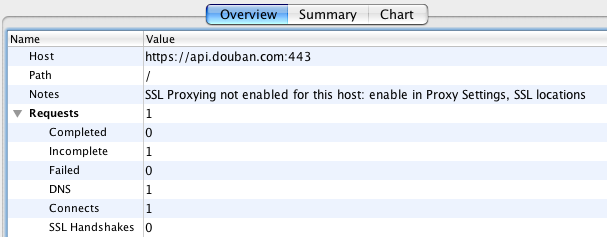
\includegraphics[scale=0.6]{charlesssltips.png}
	\caption{Charles SSL未设置代理提示}
	\label{fig:charlesssltips}
\end{figure}

需要Charles设置SSL解析。会提示首先安装CA SSL证书,其次在代理设置中启用SSL代理,设置如图\ref{fig:httpcharlesparse}所示。

\begin{figure}[htbp]
	\centering
	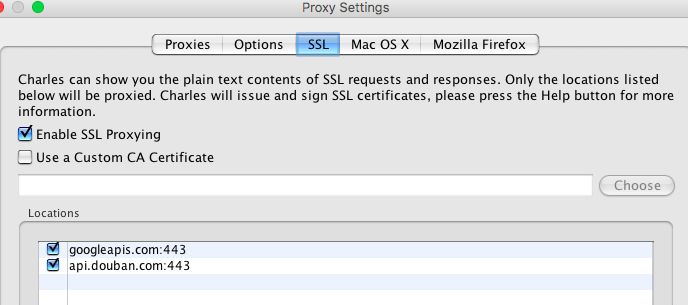
\includegraphics[scale=0.5]{httpcharlesparse.png}
	\caption{Charles设置解析网站}
	\label{fig:httpcharlesparse}
\end{figure}

设置完毕后,在每次请求时,可以在Charles中捕捉到请求,并查看应用实际的请求头。最终发现是由于设置的Agent请求头未生效导致。豆瓣对单个IP爬取数据的频率有限制,只能够降低请求对频率来获取数据。最近发现可以生成一个代理的IP池,使用免费的代理来突破爬取速度的限制,经过比较,选择了proxy\_pool\footnote{\url{https://github.com/jhao104/proxy_pool}}

\subsection{调试}

在Visual Studio中新增条件断点如图\ref{fig:visualstudiocodeconditionbeakpoint}所示。

\begin{figure}[htbp]
	\centering
	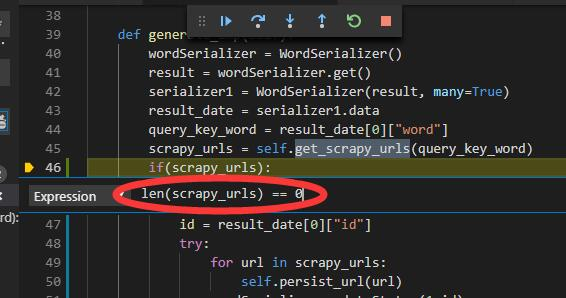
\includegraphics[scale=0.8]{visualstudiocodeconditionbeakpoint.jpg}
	\caption{Visual Studio Code条件断点}
	\label{fig:visualstudiocodeconditionbeakpoint}
\end{figure}

scrapy\_urls返回爬取网页的链接列表,list数据类型,如果列表为空,不保存。

\subsection{Unable to write settings}

在使用Visual Studio Code开发时,由于setting文件由版本管理工具Git管理时冲突,导致无法正确读取和改写配置文件。

\subsection{pipenv}

Pipenv 附带包管理和虚拟环境支持,因此你可以使用一个工具来安装、卸载、跟踪和记录依赖性,并创建、使用和组织你的虚拟环境。你的应用程序可能依赖于某个特定版本的库,而那个库可能依赖于另一个特定版本的库,这些依赖关系如海龟般堆叠起来。当你的应用程序使用的两个库有冲突的依赖关系时,你的情况会变得很艰难。Pipenv 希望通过在一个名为 Pipfile.lock 的文件中跟踪应用程序相互依赖关系树来减轻这种痛苦。Pipfile.lock 还会验证生产中是否使用了正确版本的依赖关系。pipenv的locking环节真是慢,使用下面的命令直接跳过locking环节:

\begin{lstlisting}[language=Bash]
pipenv install psycopg2 --skip-lock
\end{lstlisting}

在没有关联Python路径的情况下指定Python路径:

\begin{lstlisting}[language=Python]
pipenv install --python /usr/bin/python3
\end{lstlisting}
<<<<<<< .mine\begin{lstlisting}[language=Python]
pipenv install --python /usr/bin/python3
\end{lstlisting}

=======

>>>>>>> .theirs\subsection{Scrapy}

Scrapy需要依赖Twisted模块,Twisted模块需要依赖Visual C++\footnote{下载地址2019年1月可用,链接为:\url{https://support.microsoft.com/en-us/help/2977003/the-latest-supported-visual-c-downloads}}模块,但是进入网站却貌似没有找到独立模块的下载地址,安装Visual Studio不太现实,几个GB。这个网站\footnote{\url{https://www.lfd.uci.edu/~gohlke/pythonlibs/\#twisted}}已经有集成的包,下载集成好的包,直接离线安装即可。

\begin{lstlisting}[language=Bash]
# 离线安装Twisted
pip3 install Twisted-18.9.0-cp37-cp37m-win_amd64.whl
# 安装Scrapy
pip3 install scrapy
\end{lstlisting}

有时离线安装也会失败,可以采用源码编译的方式:


\begin{lstlisting}[language=Bash]
wget https://twistedmatrix.com/Releases/Twisted/17.1/Twisted-17.1.0.tar.bz2
tar -jxvf Twisted-17.1.0.tar.bz2
cd Twisted-17.1.0
# 多个Python版本时,指定具体版本号
python3.7 setup.py install
\end{lstlisting}


在解压tar.bz2包时,有时会提示tar (child): lbzip2: Cannot exec: No such file or directory,注意要安装依赖包bzip2。


<<<<<<< .mine\begin{lstlisting}[language=Bash]
wget https://twistedmatrix.com/Releases/Twisted/17.1/Twisted-17.1.0.tar.bz2
tar -jxvf Twisted-17.1.0.tar.bz2
cd Twisted-17.1.0
# 多个Python版本时,指定具体版本号
python3.7 setup.py install
\end{lstlisting}
=======\subsection{yield}
>>>>>>> .theirs
<<<<<<< .mine在解压tar.bz2包时,有时会提示tar (child): lbzip2: Cannot exec: No such file or directory,注意要安装依赖包bzip2。
=======yield在每次迭代中返回下一个数值,内存空间占用很小,通过 next() 不断返回数列的下一个数,内存占用始终为常数,想要保持第一版 fab 函数的简洁性,同时又要获得 iterable 的效果,yield 就派上用场了。
>>>>>>> .theirs
<<<<<<< .mine=======
>>>>>>> .theirs\subsubsection{代理池(Proxy Pool)}

一般限制了爬虫的网站,在使用同一个IP在一段时间内发送了超过规定数量的请求,或者调取速度过于频繁,会立即被加入黑名单,封禁一段时间(豆瓣一般是24小时),所以如果需要大规模抓取数据,针对此种反爬手段就是建立一个代理集合,也就是代理池,请求通过分布在全球各地的代理机器转发。HTTP代理池使用的是开源项目,新代理IP的抓取与存储,代理IP有效性的维护与检测,代理IP库对外的获取接口皆统一由开源组件来管理了。应用中需要做的就是调取对应代理服务的接口,获取一个随机的代理IP。在Scrapy中定义一个代理Middleware如下代码片段所示:

\begin{lstlisting}[language=Python]
class ProxyMiddleware(object):
    
    def process_request(self, request, spider):
      proxy_address = self.get_random_proxy()
      request.meta["proxy"]="http://" + proxy_address
\end{lstlisting}

设置代理后,\textbf{每次发送请求都会重新设置新的代理IP,不用担心多个请求发送时会被封IP},所以在使用代理的前提下可以在Scrapy爬取列表中同时设置多个请求URL,当需要大批量抓取数据时,可以调整请求URL的列表,中间的调度,可以交给Scrapy来处理,Scrapy可以方便的发送大规模的请求,而不需要费精力手动去管理线程,接收请求等,抓取到数据后,即可自动放入Pipline,可以理解为一个处理数据流的管道或者队列,在IP池足够多时,抓取的效率是非常可观的,前提是服务端能够承受大批量请求的压力。

\subsubsection{优化(Optimization)}

提高并发数量,调整settings的CONCURRENT\_REQUESTS参数。将下载延迟设为0,这时需要相应的防ban措施,一般使用user agent轮转,构建user agent池,轮流选择其中之一来作为user agent。设置DOWNLOAD\_DELAY为0,此项配置会导致服务器会在同一时刻接收到大规模集中的访问,对服务器的影响较大,相当于短时间中增大服务器负载。当代理地址响应较慢时,可以适当调低DOWNLOAD\_TIMEOUT参数,如果不设置默认是180s,那么应用会等待较长时间,会影响爬取当效率。明智的做法时快速失败,快速重试,第一个地址响应较慢,可以快速的使用另一个地址进行尝试。

\subsubsection{Json序列化}

在Scrapy爬取内容后,使用ScrapyJSONEncoder来转化为Json,再编码为bytes方式传输。ScrapyJSONEncode转化为Json:

\begin{lstlisting}[language=SQL]
_encoder = ScrapyJSONEncoder()
encode_result = _encoder.encode(data)
\end{lstlisting}

转化为bytes:

\begin{lstlisting}[language=SQL]
encode_data_bytes = urllib.parse.quote_plus(encode_result)
data = bytes(encode_data_bytes,'utf8')
req = Request(url=url,data = data,headers = headers,method='POST')
response = urllib.request.urlopen(req).read()
response_text = str(response,'utf-8')
\end{lstlisting}

\subsubsection{Spider参数传递}

在爬虫中获取爬取的关键字,将进行2次服务器端请求,所以通过参数将爬取的关键字传入爬虫。

\begin{lstlisting}[language=Python]
try:
	# This will raise an exception if scrapy fails
	# which is probably a good idea in most scenarios
	run(["scrapy", "crawl", "googlebook", "-a", "arg=" + scrapy_url],check=True)
except BaseException as e:
	logger.error(e)
\end{lstlisting}

将scrapy\_url传入Spider。注意捕获异常时是BaseException不是Exception。

\subsection{常见问题}

\subsubsection{No module named \_sqlite3}

编译时没有包含sqlite,输入如下命令安装:

\begin{lstlisting}[language=Bash]
yum -y install sqlite-devel
\end{lstlisting}

重新配置(Re-configure),重新编译(Re-compiled)Python3:

\begin{lstlisting}[language=Bash]
# 重新执行configure
./configure --enable-loadable-sqlite-extensions
# 编译
make
# 安装
make install
\end{lstlisting}

\subsubsection{callback不调用}

是因为启用了allowed\_domains设置的缘故。allowed\_domains用于设置过滤爬取的域名,在插件OffsiteMiddleware启用的情况下(默认是启用的),不在此允许范围内的域名就会被过滤,因而不会进行爬取。但对于start\_urls里的起始爬取页面,它不过滤,仅过滤起始爬取页面以外的页面。

\subsection{Google Spider}

Google书籍链接的抓取地址:https://www.googleapis.com/books/v1/volumes?q=ab,其中q表示查询的关键字。为了数据爬取,构建一个公共的词库,目前使用清华大学的开放中文词库\footnote{\url{http://thuocl.thunlp.org/sendMessage}}、OmegaWiki\footnote{\url{http://www.omegawiki.org}}。将词库导入Postgresql:


\begin{lstlisting}[language=Bash]
# 登陆dolphin数据库
psql -h 127.0.0.1 -p 5432 -d dolphin -U postgres
COPY fund_words_lib(word,remark) from '/Users/dolphin/Downloads/def_eng.csv' WITH CSV  HEADER;
# 导入词库
COPY words(word) from '/Users/dolphin/source/pydolphin-service/dolphin/tool/file.csv' WITH CSV HEADER;
\end{lstlisting}


在抓取Google API数据时,在浏览器和终端可以请求到数据,但是Scrapy的下载器却不能请求到数据,是由于浏览器和终端默认使用的Google API的IPv6地址,而Scrapy目前未支持IPv6导致,IPv4无法直接访问Google服务\footnote{\url{https://github.com/scrapy/scrapy/issues/3528}}.Google Book API\footnote{\url{https://developers.google.com/books/docs/v1/reference/volumes/list?hl=zh-CN}}支持翻页,每页最大40条数据。Google Book不同的IP调用返回的结果不同,不同的分页参数返回的结果总数不同。

\subsubsection{速度限制}

Google API使用令牌桶算法来衡量请求数并确定每秒查询数 (QPS) 速率。这样做的目的是阻止恶意的或不可控的软件大量调用API服务器,影响其他用户。例如,如果某个失控的客户端意外产生数以千计的线程来同时调用API,API 服务器就会在发现后返回一个 RateExceededError,要求调用软件减速。

\subsubsection{xpath}

XPath为XML路径语言(XML Path Language),它是一种用来确定XML文档中某部分位置的语言。简单示例如下:

\begin{lstlisting}[language=Python]
sites = sel.xpath('//*[@id="detail_bullets_id"]/table/tr/td/div/ul/li') 
\end{lstlisting}

以上表达式过滤出亚马逊商品的详细列表信息,双斜杠加星号表示选取文档中的所有元素,@表示选取属性,需要加上中括号。


\subsection{api}

启动爬虫接口服务端的命令如下:

\begin{lstlisting}[language=Bash]
# 启动API应用,服务端监听端口为9000
/usr/local/bin/python3 manage.py runserver 0.0.0.0:9000
\end{lstlisting}


POST请求接口:

\begin{lstlisting}[language=Bash]
curl -H "Content-Type:application/json" -X POST --data '{"index":"true"}' http://localhost:8000/spider/api/book
\end{lstlisting}

body传送json数据:

\begin{lstlisting}[language=Bash]
curl -XPOST -H’Content-Type: application/json’ http://localhost:8000/spider/api/book -d@temp.json
python3 manage.py runserver 0.0.0.0:9000
\end{lstlisting}

服务端接收请求:

\begin{lstlisting}[language=Bash]
location ^~ /spider/api/ {
	# 匹配爬虫服务URL
	# 匹配符合以后,停止往下搜索正则,采用这一条
	proxy_pass http://spider-service;
}
\end{lstlisting}

\paragraph{JsonResponse}

第一个参数,data应该是一个字典类型,当 safe 这个参数被设置为:False ,那data可以填入任何能被转换为JSON格式的对象,比如list, tuple, set。 默认的safe 参数是 True. 如果你传入的data数据类型不是字典类型,那么它就会抛出 TypeError的异常。在返回Json响应的时候,一般不会直接返回查询出来的结果,要进行一次简单的标准化封装,返回如下格式的数据:

\begin{lstlisting}
{
    "code": "20000",
    "data": {},
    "message": "success"
}
\end{lstlisting}

通过新增自定义响应CustomJsonResponse,封装成标准化的响应结果,效果如图\ref{fig:pythonreststandardresponse}所示。

\begin{figure}[htbp]
	\centering
	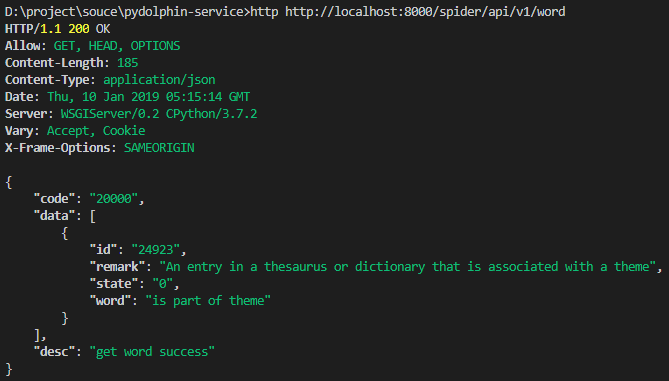
\includegraphics[scale=0.7]{pythonreststandardresponse.png}
	\caption{Django自定义标准化Json响应}
	\label{fig:pythonreststandardresponse}
\end{figure}


http http://localhost:8000/spider/api/v1/word

\paragraph{'utf8' codec can't decode byte 0x8b in position 1: invalid start byte}

由于默认请求头包含gzip格式,服务端在返回的时候,对消息体进行了压缩。客户端发送Accept-Encoding请求头表示接收的内容类型。Python默认不自动解压,无法识别,所以出现此问题。

\begin{lstlisting}
'Accept-Encoding':'gzip, deflate, br',
\end{lstlisting}

去掉gzip压缩类型即可。

\section{Django}

\subsection{使用事务(Using Transaction)}

在爬取数据获取爬取链接时,由于同步运行有多个客户端,为了避免客户端获取到相同的链接,需要在查询接口中开启事务来避免此种情况。

\begin{lstlisting}[language=Python]
# Avoid multi spider get the same key word
# Make each query atomic
# Pay attention the performance issue by transaction
@transaction.atomic
def get(self,request):
	serializer = WordSerializer()
	result = serializer.get()
	serializer1 = WordSerializer(result, many=True)
	return  CustomJsonResponse(data=serializer1.data, code="20000", desc='get word success' )
  
\end{lstlisting}

\subsection{PgBouncer}

PgBouncer是一个针对PostgreSQL数据库的轻量级连接池,任何目标应用都可以把PgBouncer当作一个 PostgreSQL 服务器来连接,然后PgBouncer会处理与服务器连接,或者是重用已存在的连接。PgBouncer的目标是降低因为新建到PostgreSQL的连接而导致的性能损失。为了在Google Cloud PostgreSQL限制数据库连接数的情况下,尽可能的提高数据库连接的效率,引入PgBouncer连接池组件。安装PgBouncer之前需要先安装libevent。

\begin{lstlisting}[language=Bash]
# 安装依赖
yum install -y openssl openssl-devel libevent-devel python-docutils libtool automake autoconf
# 安装libevent
./configure --prefix=/home/pgsql/libevent
# 安装PgBouncer
./configure --prefix=/home/pgsql/pgbouncer/ --with-libevent=/home/pgsql/libevent/ 
# 启动PgBouncer
/home/pgsql/pgbouncer/bin/pgbouncer -d /etc/pgbouncer/pgbouncer.ini
\end{lstlisting}

提示错误FATAL @src/main.c:913 in function main(): unix socket is in use, cannot continue。这个报错是套接字还在使用导致的启动失败,因为pgbouncer是可以socket连接,所以一般会有一个socket文件,通常这个文件默认在/tmp下面,一般以端口号码结尾,删除这个socket文件,再启动就正常。

\section{日志中心(Logging Center)}

根据 Google Trend 的信息显示,ELK Stack已经成为目前最流行的集中式日志解决方案。ELK的整体流程如图\ref{fig:elklogarchitecture}所示。




\begin{figure}[htbp]
	\centering
	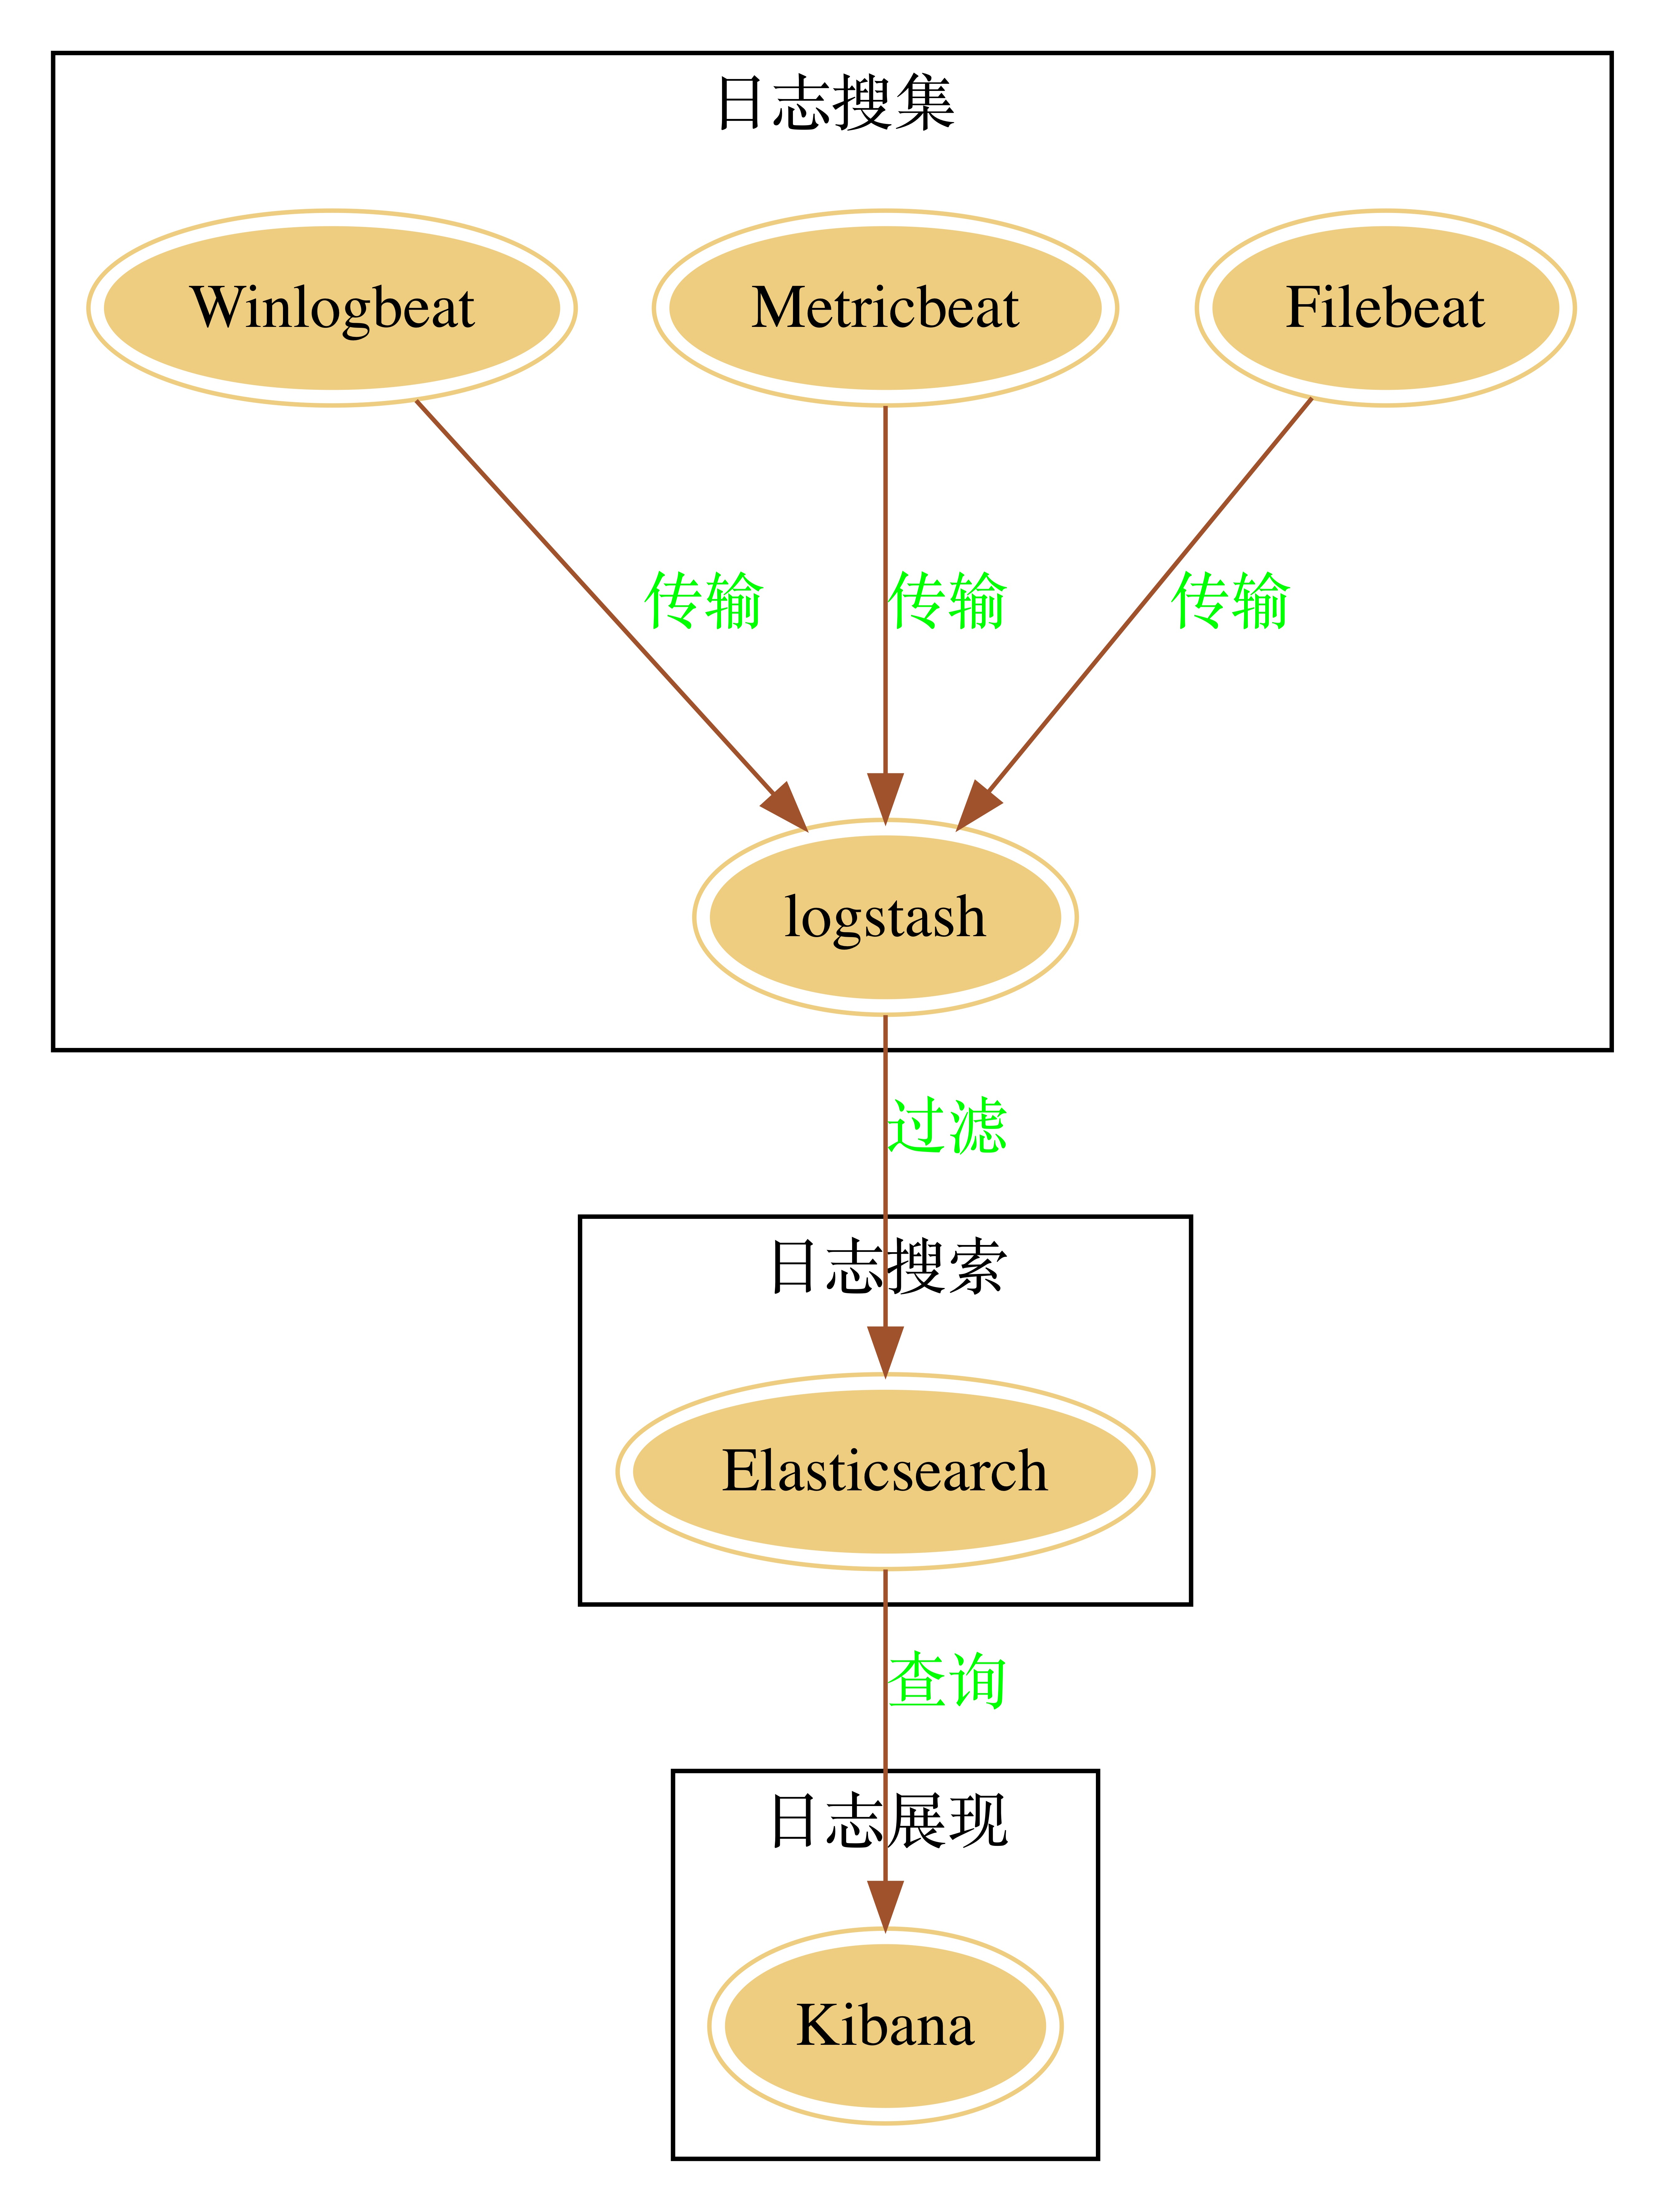
\includegraphics[scale=0.05]{elk-log-architecture.jpg}
	\caption{ELK流程}
	\label{fig:elklogarchitecture}
\end{figure}
logstash数据收集引擎。它支持动态的从各种数据源搜集数据,并对数据进行过滤、分析、丰富、统一格式等操作,然后存储到用户指定的位置。Logstash 项目诞生于 2009 年 8 月 2 日。其作者是世界著名的运维工程师乔丹西塞(JordanSissel),乔丹西塞当时是著名虚拟主机托管商 DreamHost 的员工,还发布过非常棒的软件打包工具 fpm,并主办着一年一度的 sysadmin advent calendar(advent calendar 文化源自基督教氛围浓厚的 Perl 社区,在每年圣诞来临的 12 月举办,从 12 月 1 日起至 12 月 24 日止,每天发布一篇小短文介绍主题相关技术)。logstash是jvm跑的,资源消耗比较大,启动一个logstash就需要消耗500M左右的内存,而filebeat只需要10来M内存资源。Filebeat轻量型日志采集器。当您要面对成百上千、甚至成千上万的服务器、虚拟机和容器生成的日志时,Filebeat 将为您提供一种轻量型方法,用于转发和汇总日志与文件,让简单的事情不再繁杂。查看Elastic配置:

\begin{lstlisting}[language=Bash]
curl -XGET -H "Content-Type: application/json" http://localhost:9200/_all/_settings|jq '.'
\end{lstlisting}

修改Elastic配置:

\begin{lstlisting}[language=Bash]
curl -XPUT -H "Content-Type: application/json" http://localhost:9200/_all/_settings 
-d '{"index.blocks.read_only_allow_delete": null}'
\end{lstlisting}

对日志统一格式定义如下:


\begin{lstlisting}
{
	"date": "yyyy - MM - dd HH: mm: ss ",
	"ip/host" "192.168.1.12",
	"pid": "1211",
	"topic": "track"
	"type": "error",
	"tag": "redis connection refused",
	"platform": "java/go/php",
	"level": "info/warn/error",
	"app": "appName",
	"module": "com.youzan.somemodule",
	"detail": "any things you want here"
}
\end{lstlisting}

\section{配置管理中心(Configuration Management Center)}

随着程序功能的日益复杂,程序的配置日益增多:各种功能的开关、参数的配置、服务器的地址。并且有对配置的各类要求,配置修改后实时生效,灰度发布,分环境、分集群管理配置,完善的权限、审核机制。并且随着采用分布式的开发模式,项目之间的相互引用随着服务的不断增多,相互之间的调用复杂度成不断升高,因此需要引用配置中心治理。常用的配置管理工具有:

\begin{table}[htbp]
	\caption{配置管理工具}
	\label{table:configmanagementtool}
	\begin{center}
		\begin{tabular}{|c|c|p{8cm}|}
			\hline
			\multirow{1}{*}{工具名称}
			& \multicolumn{1}{c|}{开发语言} 
			& \multicolumn{1}{c|}{备注}\\			
			\cline{1-3}
			etcd &  Go  & 分布式键值存储,用于共享配置和服务发现 \\
			\hline
			consul & Go &  一款服务发现和配置的工具 \\
			\hline
			Doozer & Go & 分布式的一致性数据存储服务 \\
			\hline							
		\end{tabular}	
	\end{center}
\end{table}

etcd是由CoreOS开发并维护的,灵感来自于ZooKeeper和Doozer,它使用Go语言编写,并通过Raft一致性算法处理日志复制以保证强一致性。 Raft是一个来自Stanford的新的一致性算法。


\begin{table}[htbp]
	\caption{配置管理工具}
	\label{table:configmanagementtool}
	\begin{center}
		\begin{tabular}{|c|c|p{8cm}|}
			\hline
			\multirow{1}{*}{工具名称}
			& \multicolumn{1}{c|}{开发语言} 
			& \multicolumn{1}{c|}{备注}\\			
			\cline{1-3}
			etcd &  Go  & 分布式键值存储,用于共享配置和服务发现 \\
			\hline
			consul & Go &  一款服务发现和配置的工具 \\
			\hline
			Doozer & Go & 分布式的一致性数据存储服务 \\
			\hline							
		\end{tabular}	
	\end{center}
\end{table}

etcd是由CoreOS开发并维护的,灵感来自于ZooKeeper和Doozer,它使用Go语言编写,并通过Raft一致性算法处理日志复制以保证强一致性。 Raft是一个来自Stanford的新的一致性算法。



\begin{figure}[htbp]
	\centering
	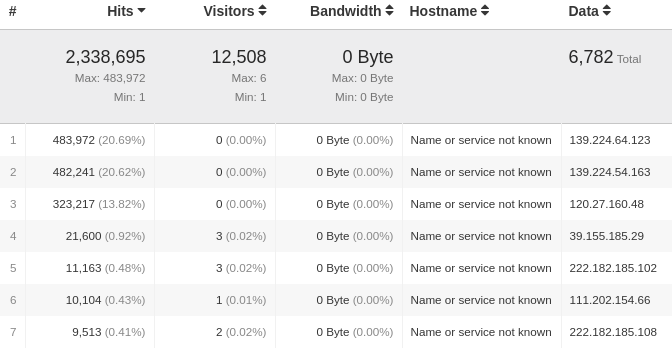
\includegraphics[scale=0.4]{ipstatistics.png}
	\caption{根据IP统计}
	\label{fig:ipstatistics}
\end{figure}


\begin{figure}[htbp]
	\centering
	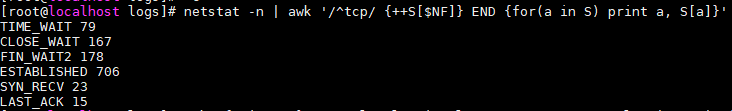
\includegraphics[scale=0.5]{websiteconcurrentaccess.png}
	\caption{查看服务器并发示例}
	\label{fig:websiteconcurrentaccess}
\end{figure}

\begin{figure}[htbp]
	\centering
	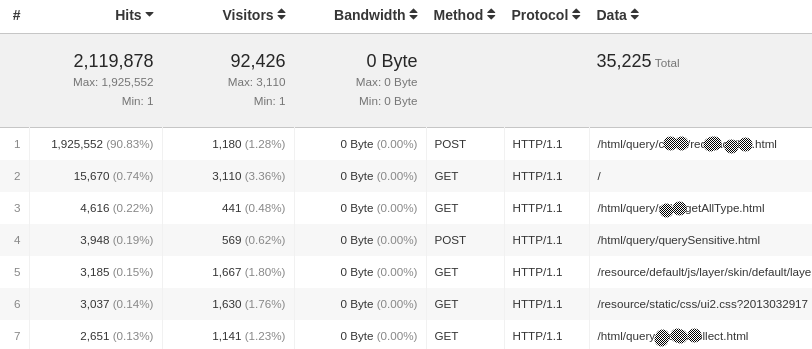
\includegraphics[scale=0.35]{spideranalysis.png}
	\caption{访问URL统计}
	\label{fig:spideranalysis}
\end{figure}

\begin{figure}[htbp]
	\centering
	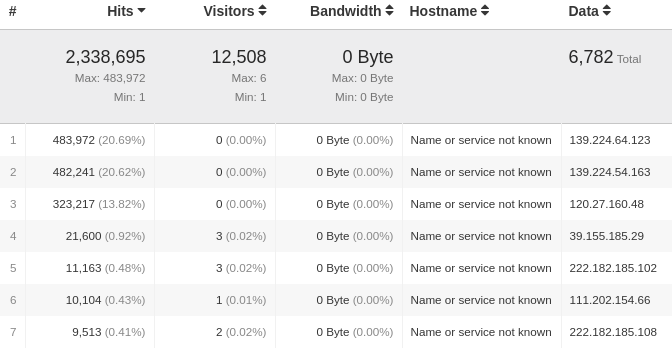
\includegraphics[scale=0.4]{ipstatistics.png}
	\caption{根据IP统计}
	\label{fig:ipstatistics}
\end{figure}

\begin{figure}[htbp]
	\centering
	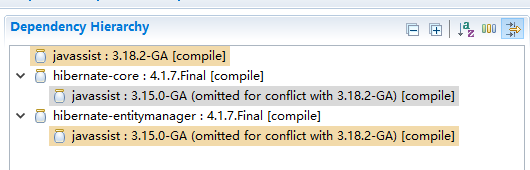
\includegraphics[scale=0.7]{dependencyconflict.png}
	\caption{依赖冲突}
	\label{fig:dependencyconflict}
\end{figure}

\section{监控中心(Monitor Center)}


\chapter{MQ(Message Queue)}

\section{Apache Kafka}

\subsection{基础概念}

\paragraph{Rebalance}

在某些条件下,partition要在consumer中重新分配。以下条件,会触发rebalance:有新的consumer加入,旧的consumer挂了,coordinator挂了,集群选举出新的coordinator,topic的partition新加,consumer调用unsubscrible(),取消topic的订阅。当consumers检测到要rebalance时,所有consumer都会重走上面的流程,进行步骤JoinGroup + SyncGroup。当一个consumer挂了,或者有新的consumer加入,其他consumers通过heartbeat知道要进行rebalance。

\subsection{分区(Partition)}

ProducerRecord 对象包含了目标主题、键和值。 Kafka的消息是一个个键值对, ProducerRecord对象可以只包含目标主题和值,键可以设置为默认的 null,不过大多数应用程序会用到键。键有两个用途 :可以作为消息的附加信息,也可以用来决定消息该被写到主题的哪个分区。拥有相同键的悄息将被写到同一个分区。

\subsection{Producer}

创建生产者提示kafka.errors.NoBrokersAvailable exception。此时需要配置服务端server.properties:

\begin{lstlisting}[language=Bash]
# Hostname and port the broker will 
# advertise to producers and consumers. 
# If not set, it uses the value for "listeners" if configured.  
# Otherwise, it will use the value returned from 
# java.net.InetAddress.getCanonicalHostName().
# 这里配置的地址要保证生产者和消费者能够直接访问
advertised.listeners=PLAINTEXT://10.142.0.2:9092
\end{lstlisting}

advertised监听的配置是有讲究的,掉这个坑里面整整一天。这个配置是生产者和消费者需要使用的,开始的时候配置的是内网的地址,这就出问题了,生产者拿到这个配置后一直向内网IP发送消息,由于Kafka部署在Google云上,机器在美国,根本不在同一个局域网,肯定是无法发送成功的,导致生产者一直超时,无法获取到元数据。所以这里需要配置公网的IP地址,调整后即可解决问题。如果没有设置,将会使用listeners的配置,如果listeners也没有配置,将使用java.net.InetAddress.getCanonicalHostName()来获取这个hostname和port。将localhost调整为IP后,服务端消费时提示Broker may not be available,是由于为了支持外部访问Kafka,server.propertise文件中指定绑定IP,此时生产消费脚本也需要通过IP来进行。advertised.listeners为Kafka 0.9.x以后的版本新增配置,原来的advertise.host.name和port配置不建议再使用。同时在Python初始化的时候添加API版本参数。

\begin{lstlisting}[language=Python]
producer = KafkaProducer(
  bootstrap_servers=['mq-server:9092'],
  api_version_auto_timeout_ms=10000,
  # fix no broker avaliable problem
  api_version = (0, 10)
)
\end{lstlisting}

出现此错误KafkaTimeoutError('Failed to update metadata after 60.0 secs.')是由于Python的Kafka客户端版本不匹配,服务端安装的是最新的2.x版本,而客户端最高支持1.1版本,所以会出现此问题,降低服务端版本即可解决此问题。使用命令创建Topic:

\begin{lstlisting}[language=Bash]
bin/kafka-topics.sh --create --zookeeper localhost:2181 --replication-factor 1 --partitions 1 --topic dolphin-test
\end{lstlisting}

安装完成后,可以启动消费者,再使用生产者脚本发送信息,在消费端查看输出,即可验证Kafka:

\begin{lstlisting}[language=Bash]
# 消费dolphin-test主题消息
bin/kafka-console-consumer.sh --bootstrap-server 10.142.0.2:9092 --topic dolphin-spider-google-book-bookinfo --from-beginning
# 生产dolphin-test主题消息
bin/kafka-console-producer.sh --broker-list 10.142.0.2:9092 --topic dolphin-test
\end{lstlisting}

测试Kafka消息生产与消费过程如图\ref{fig:kafkasendingmessagetest}所示,生产者向主题dolphin-test发送Hello,Dolphin!消息,消费者消费到此条消息:

\begin{figure}[htbp]
	\centering
	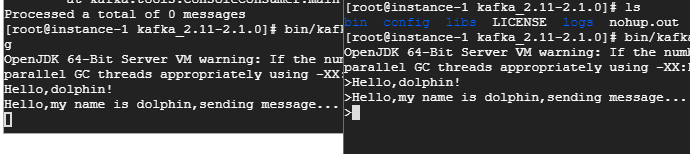
\includegraphics[scale=0.7]{kafkasendingmessagetest.png}
	\caption{Kafka发送消息测试}
	\label{fig:kafkasendingmessagetest}
\end{figure}

\subsubsection{Key}

Kafka发送消息时,key可以不用指定。如果不指定消息的key,则消息发送到的分区是随着时间不停变换的。如果指定了消息的key,则会根据消息的hash值和topic的分区数取模来获取分区的。如果应用有消息顺序性的需要,则可以通过指定消息的key和自定义分区类来将符合某种规则的消息发送到同一个分区。同一个分区消息是有序的,同一个分区只有一个消费者就可以保证消息的顺序性消费。

\begin{lstlisting}[language=Python]
log.segment.bytes=536870912
log.retention.check.interval.ms=60000
log.cleaner.enable=false
# 数据文件保留多长时间
# log.retention.bytes
# log.retention.minutes
# log.retention.hours任意一个达到要求,都会执行删除
log.retention.minutes=300
log.retention.hours=24
\end{lstlisting}



\subsection{Consumer}

Kafka消费者Python客户端如下代码片段所示(不同Kafka版本略有区别):


\begin{lstlisting}[language=Python]
consumer = KafkaConsumer('dolphin-test',
                         bootstrap_servers=['mq-server:9092'],
                         group_id = "console-consumer-30308",
                         consumer_timeout_ms=5000)

def consume_bookinfo(self):
    while True:        
        for msg in self.consumer:
            recv = "%s:%d:%d: key=%s value=%s" % (msg.topic, msg.partition, msg.offset, msg.key, msg.value)
            print(recv)
\end{lstlisting}

console-consumer-30308表示消费控制台组的消息,可以使用命令将消息推送到控制台,在代码中使用客户端获取,调试消费着非常方便,参数group\_id必须要指定。dolphin-test是消息的主题。Java版本的消费者客户端如下代码片段所示:

\begin{lstlisting}[language=Java]
Properties props = new Properties();
props.put("bootstrap.servers", "mq-server:9092");
props.put("group.id", "console-consumer-30308");
props.put("enable.auto.commit", "true");
props.put("auto.commit.interval.ms", "1000");
props.put("key.deserializer", "org.apache.kafka.common.serialization.StringDeserializer");
props.put("value.deserializer", "org.apache.kafka.common.serialization.StringDeserializer");
KafkaConsumer<String, String> consumer = new KafkaConsumer<>(props);
consumer.subscribe(Arrays.asList("dolphin-test", "dolphin-spider-google-book-bookinfo"));
while (true) {
    ConsumerRecords<String, String> records = consumer.poll(100);
    for(ConsumerRecord<String, String> record :records){
       System.out.println("value:" + record.value());
    }
}
\end{lstlisting}

group.id是一个字符串,唯一标识一个Consumer Group。多个消费者或消费者实例(Consumer Instance),它们共享一个公共的ID,即Group ID。组内的所有消费者协调在一起来消费订阅主题(Subscribed Topics)的所有分区(Partition)。当然,每个分区只能由同一个消费组内的一个Consumer来消费。在Consumer中可以自定义Group ID(不需要Producer生产数据时指定),当Consumer消费数据后,Group ID自动注册到服务端。使用如下命令查看当前Group ID有哪些Topic:

\begin{lstlisting}[language=Bash]
bin/kafka-consumer-groups.sh --bootstrap-server mq-server:9092 --describe --group google-book
\end{lstlisting}

\subsubsection{提高消费能力-多线程}

接收到信息后,交给独立的线程处理:

\begin{lstlisting}[language=Python]
def sub_process_handle(self,bookinfo):     
    number_of_threadings = len(threading.enumerate())
    if(number_of_threadings < 15):
        t = threading.Thread(target=self.background_process, args=(bookinfo,), kwargs={})
        t.start()
    else:
        # If all threading running
        # Using main thread to handle
        # Slow down kafka consume speed
        self.parse_bookinfo(bookinfo)
\end{lstlisting}

注意线程开启较多之后,需要增大数据库Session数量,Google Cloud限制了PostgreSQL的最大连接数量,真是恼火,线程增加后出现此错误OperationalError('FATAL:  remaining connection slots are reserved for non-replication superuser connections')。

\subsubsection{提高消费能力-多消费者}

也可以提高Partition数量,从而提高Consumer的并行能力,从而提高数据的消费能力,不过目前Google Cloud数据库实例对PostgreSQL最大会话的限制(25个)会成为瓶颈。Topic下的一个分区只能被同一个Consumer Group下的一个Consumer线程来消费。为了实现传统Message Queue消息只被消费一次的语义,Kafka保证每条消息在同一个Consumer Group里只会被某一个Consumer消费。与传统Message Queue不同的是,Kafka还允许不同Consumer Group同时消费同一条消息,这一特性可以为消息的多元化处理提供支持。

\subsection{常用命令}

查看所有Topic的信息:

\begin{lstlisting}[language=Bash]
# 启动Kafka
bin/kafka-server-start.sh config/server.properties

# 启动Zookeeper
bin/zookeeper-server-start.sh config/zookeeper.properties

bin/kafka-topics.sh --zookeeper localhost:2181 --list

# 查看当前Broker中的所有组
bin/kafka-consumer-groups.sh --bootstrap-server mq-server:9092 --list

# 查看主题dolphin-spider-google-book-bookinfo信息
bin/kafka-topics.sh --zookeeper localhost:2181 --describe --topic dolphin-spider-google-book-bookinfo

# 查看消费组google-book情况
bin/kafka-consumer-groups.sh --bootstrap-server localhost:9092 --describe --group google-book
\end{lstlisting}

查看消费堆积情况语句如下:

\begin{lstlisting}[language=Bash]
# 查看Kafka消息堆积情况
/home/dolphin/software/kafka_2.12-1.1.0/bin/kafka-consumer-groups.sh --bootstrap-server mq-server:9092 --group google-book --describe
\end{lstlisting}

输出结果如图\ref{fig:kafkaconsumecheck}所示,输出的内容可以知道消息主题是dolphin-spider-google-book-bookinfo,消息属于0分区(Partition),当前消费到第761条数据,总共有1386条数据,还有625条数据未消费(Lag Behand),消费者ID是dolphin-pipline-google-bookinfo-consumer-foolman-fe57df81-6dea-45                                                                    b6-a6f4-8972386a24ec,客户端ID是dolphin-pipline-google-bookinfo-consumer-foolman。

\begin{figure}[htbp]
	\centering
	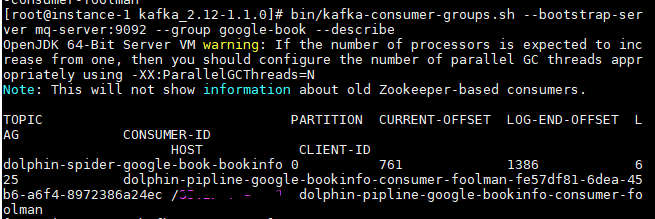
\includegraphics[scale=0.7]{kafkaconsumecheck.png}
	\caption{Kafka消费情况查看}
	\label{fig:kafkaconsumecheck}
\end{figure}

重置offset:

\begin{lstlisting}[language=Bash]
/home/dolphin/software/kafka_2.12-1.1.0/bin/kafka-consumer-groups.sh --bootstrap-server mq-server:9092 --group google-book --topic dolphin-spider-google-book-bookinfo --reset-offsets --to-earliest --execute
\end{lstlisting}




\subsection{配置}

\paragraph{max.poll.interval.ms}

Kafka消费者在会保存其消费的进度,也就是offset,存储的位置根据选用的kafka api不同而不同。消费者在创建时会有一个属性max.poll.interval.ms,该属性意思为kafka消费者在每一轮poll()调用之间的最大延迟,消费者在获取更多记录之前可以空闲的时间量的上限。如果此超时时间期满之前poll()没有被再次调用,则消费者被视为失败,并且分组将重新平衡,以便将分区重新分配给别的成员。kafkaConsumer调用一次轮询方法只是拉取一次消息。客户端为了不断拉取消息,会用一个外部循环不断调用消费者的轮询方法。每次轮询到消息,在处理完这一批消息后,才会继续下一次轮询。但如果一次轮询返回的结构没办法及时处理完成,会有什么后果呢?服务端约定了和客户端max.poll.interval.ms,两次poll最大间隔。如果客户端处理一批消息花费的时间超过了这个限制时间,服务端可能就会把消费者客户端移除掉,并触发rebalance。

\paragraph{auto\_offset\_reset}

earliest:当各分区下有已提交的offset时,从提交的offset开始消费;无提交的offset时,从头开始消费。latest:当各分区下有已提交的offset时,从提交的offset开始消费;无提交的offset时,消费新产生的该分区下的数据。none:topic各分区都存在已提交的offset时,从offset后开始消费;只要有一个分区不存在已提交的offset,则抛出异常。注意一般情况下设置为earliest,设置为latest会忽略掉未消费的数据,直接从最新产生的消息进行消费,同时offset也会默认更新为最新。


\paragraph{消息过期}

对于传统的message queue而言,一般会删除已经被消费的消息,而Kafka集群会保留所有的消息,无论其被消费与否。当然,因为磁盘限制,不可能永久保留所有数据(实际上也没必要),因此Kafka提供两种策略去删除旧数据。一是基于时间,二是基于partition文件大小。例如可以通过配置\$KAFKA\_HOME/config/server.properties,让Kafka删除一周前的数据,也可通过配置让Kafka在partition文件超过1GB时删除旧数据。

\subsection{常见问题}

\subsubsection{Commit cannot be completed since the group has already rebalanced}

kafka设置了自动提交,但在规定的提交时间之内却没有处理完消息,导致消息自动提交出错,这样还会引发一个问题,就是当提交的消息不成功,kafka有重试机制,这样就会重新消费该消息,但消费又不成功,这样循环,会导致后面的消息堆积过多。在Consumer上调整消费者最大心跳时间间隔:

\begin{lstlisting}[language=Bash]
max_poll_interval_ms = 6000000
\end{lstlisting}
 
出现此问题最大的问题是消费者(Consumer)的消费能力不足,提交Offset的周期太长。可以增加Session的过期时间(session\_timeout\_ms),但是最终的解决方案应该想办法提高消费端的消费能力。    

\subsubsection{Heartbeat session expired, marking coordinator dead}

提交Kafka Offset时,提示CommitFailedError: Commit cannot be completed since the group has already rebalanced and assigned the partitions to another member.This means that the time between subsequent calls to poll() was longer than the configured max\_poll\_interval\_ms, which typically implies that the poll loop is spending too much time message processing. You can address this either by increasing the rebalance timeout with max\_poll\_interval\_ms,or by reducing the maximum size of batches returned in poll() with max\_poll\_records.大概是由于Kafka消费者与心跳之间产生了死锁\footnote{\url{https://github.com/dpkp/kafka-python/issues/1544}},不过死锁问题已经在1.4.4版本中修复,但是还是遇到了此问题\footnote{\url{https://github.com/dpkp/kafka-python/pull/1628}}。订阅一组topic后,当调用poll(long)时,消费者将自动加入到组中。只要持续的调用poll,消费者将一直保持可用,并继续从分配的分区中接收消息。此外,消费者向服务器定时发送心跳。如果消费者崩溃或无法在session.timeout.ms配置的时间内发送心跳,则消费者将被视为死亡,并且其分区将被重新分配。消费可能遇到“活锁(livelock)”的情况,它持续的发送心跳,但是没有处理。为了预防消费者在这种情况下一直持有分区,使用max.poll.interval.ms活跃检测机制。在此基础上,如果调用的poll的频率大于最大间隔,则客户端将主动地离开组,以便其他消费者接管该分区。发生这种情况时,offset出现提交失败(调用commitSync()引发的CommitFailedException)。这是一种安全机制,保障只有活动成员能够提交offset。所以要留在组中,必须持续调用poll。将消费者调整为poll的方式解决此问题:

\begin{lstlisting}[language=Python]
msg_pack = self.consumer.poll(timeout_ms=5000,max_records=1)
for messages in msg_pack.items():
    for message in messages:
        if(isinstance(message,TopicPartition)):
            logger.info("TopicPartition: %s", TopicPartition)
\end{lstlisting}

\chapter{OS}

\section{Linux}

\subsection{环境变量(Environment Variable)}

在使用云环境时环境变量优先写在当前用户下的profile文件中,避免写到全局的profile中,因为在使用远程ssh时,局部profile不太会影响到全局应用,一旦由于全局profile设置不当导致ssh启动失败,后续就比较麻烦,。

\subsection{命令}

查找大文件:

\begin{lstlisting}[language=Bash]
find / -type f -size +800M -print0 | xargs -0 du -h | sort -nr
\end{lstlisting}

查找操作系统中大于800MB的文件。让find在打印出一个文件名之后接着输出一个NULL字符 ('\textbackslash 0') 而不是换行符, 然后再告诉xargs也用NULL字符来作为记录的分隔符。

\part{Tool}

\chapter{Widgets}

\section{Little Tool}

\subsection{Shadowsocks}

当前Shadowsocks有多个实现支持,以自由软件形式发布的主要有原始Shadowsocks(以Python语言编写)、Shadowsocks-libev(分支项目openwrt-Shadowsocks)、Shadowsocks-rust、Shadowsocks-go/go-Shadowsocks2、libQtShadowsocks、Shadowsocks-qt5(仅作为客户端)、Shadowsocks-android(仅作为客户端)、Shadowsocks-windows(仅作为客户端)、ShadowsocksX-NG(仅作为客户端)、Outline、V2Ray、Brook等等,还有为数甚多的免费软件及专有软件(多数是iOS上运行的,如shadowrocket、Surge等),如下是服务端的配置示例。

\begin{lstlisting}
{
	"server":"0.0.0.0",
	"server_port":1080,
	"local_address":"127.0.0.1",
	"local_port":1080,
	"password":"password",
	"timeout":300,
	"method":"aes-256-cfb"
}
\end{lstlisting}

CFB模式(密文反馈:Cipher feedback),CFB能够将块密文(Block Cipher)转换为流密文(Stream Cipher)。ShadowSocks现在主流的加密方式有两种:aes-256-cfb 和 rc4-md5 前者加密强度高(指的并不是安全性高而是更难被 GFW 检测出来)
但系统开销会更大一点,它是很多一键包默认的加密方式,
后者加密解密速度比前者快得多,但安全性不够。如果是用在路由器上,因为很多路由器 CPU 速度都在 500MHz 以下,性能并不强,
使用 aes-256-cfb 多出来的那点性能开销在路由器上可能会构成一个影响性能的大问题,
所以,之前使用在路由器上的加密方式一般都选 rc4-md5。


\subsection{Scoop}

scoop\footnote{\url{https://github.com/lukesampson/scoop}}是 windons 下一款比较不错的安装包管理工具,试了下可以在Windows下一行命令安装curl/jq/wget等包,相当好用。

\subsection{WinDirStat}

WinDirStat\footnote{\url{https://windirstat.net/}} is a disk usage statistics viewer and cleanup tool for various versions of Microsoft Windows.
Note: if you are looking for an alternative for Linux, you are looking for KDirStat (apt-get install kdirstat or apt-get install k4dirstat on Debian-derivatives) or QDirStat and for MacOS X it would be Disk Inventory X or GrandPerspective\footnote{\url{http://grandperspectiv.sourceforge.net/}}.WinDirStat可以方便的分析出当前磁盘的使用情况,找出磁盘占用较大的文件,不同的文件类型会以不同的颜色进行区分,不同的文件大小会以不同颜色块的大小进行识别。

\subsection{traceroute}

通过traceroute我们可以知道信息从计算机到互联网另一端的主机是走的路由路径。Traceroute 程序的设计是利用ICMP及IP header的TTL(Time To Live)栏位(field)。首先,traceroute送出一个TTL是1的IP datagram(其实,每次送出的为3个40字节的包,包括源地址,目的地址和包发出的时间标签)到目的地,当路径上的第一个路由器 (router)收到这个datagram时,它将TTL减1。此时,TTL变为0了,所以该路由器会将此datagram丢掉,并送回一个 「ICMP time exceeded」消息(包括发IP包的源地址,IP包的所有内容及路由器的IP地址),traceroute 收到这个消息后, 便知道这个路由器存在于这个路径上,接着traceroute 再送出另一个TTL是2 的datagram,发现第2 个路由器...... 。traceroute 每次将送出的datagram的TTL 加1来发现另一个路由器,这个重复的动作一直持续到某个datagram 抵达目的地。当datagram到达目的地后,该主机并不会送回ICMP time exceeded消息,因为它已是目的地了,那么 traceroute如何得知目的地到达了呢?Traceroute 在送出UDP datagrams到目的地时,它所选择送达的port number 是一个一般应用程序都不会用的号码(30000 以上),所以当此 UDP datagram 到达目的地后该主机会送回一个「ICMP port unreachable」的消息,而当traceroute 收到这个消 息时,便知道目的地已经到达了。所以traceroute 在Server端也是没有所谓的Daemon程式。
Traceroute提取发ICMP TTL到期消息设备的IP地址并作域名解析。每次 ,Traceroute都打印出一系列数据,包括所经过的路由设备的域名及 IP地址,三个包每次来回所花时间。查看ipv6的路由路径(常用IPv6地址\footnote{\url{https://raw.githubusercontent.com/lennylxx/ipv6-hosts/master/hosts}}):


\begin{lstlisting}[language=Bash]
# Google公共IPv6 DNS地址1
# 2001:4860:4860::8844(google-public-dns-a.google.com)
# Google公共IPv6 DNS地址2
# google-public-dns-a.google.com
traceroute6 2001:4860:4860::8888
\end{lstlisting}
     

\subsection{dig}

dig 命令最典型的用法就是查询单个主机的信息。dig is a flexible tool for interrogating DNS name servers。

\begin{lstlisting}[language=Bash]
# 查询Google的IPv6地址
dig www.google.com AAAA
# 查询baidu的IPv6地址
dig ipv6.baidu.com AAAA
# host命令查看IPv6地址
host -t AAAA www.google.com
\end{lstlisting}


AAAA表示查看对应域名的IPv6地址。也可以通过ping6命令查看对应的IPv6地址:

\begin{lstlisting}[language=Bash]
# 查询baidu的IPv6地址
ping6 ipv6.baidu.com
# 查看Google API的IPv6地址
# 2404:6800:4005:802::200a
ping6 https://www.googleapis.com
# Wireshark过滤IPv6流量
ipv6 and ipv6.addr==2404:6800:4005:80b::200a
\end{lstlisting}

输出PING6(56=40+8+8 bytes) local ip --> 2400:da00:2::29。local ip是本机的IPv6地址。


\subsection{ssh}

使用如下命令动态代理:

\begin{lstlisting}[language=Bash]
# ssh利用Google云主机动态代理
ssh -Nf -D 127.0.0.1:2000 google-cloud
# 链接到192.168.1.11的流量转发到192.168.0.14
ssh -g -fN -L 8100:192.168.0.14:8100 192.168.1.11
\end{lstlisting}

服务端有大量拒绝连接输出,且部分网站无法正常访问,不知原因在何处。访问腾讯视频时,提示所在地区无法访问,可能是国外相应的服务封锁了部分地区的IP。

\subsubsection{ssh登录Google Cloud}

需要打开允许ssh登录、允许密码登录选项:

\begin{lstlisting}[language=Bash]
# 允许通过密码登录(不安全)
PasswordAuthentication yes
# 允许root用户登录(不安全)
PermitRootLogin yes
\end{lstlisting}

\subsubsection{ssh重启失败}

使用命令查看状态时一直停留在activating状态,是由于selinux导致,临时关闭selinux即可。

\begin{lstlisting}[language=Bash]
# 查看SELinux状态
/usr/sbin/sestatus -v
# 关闭SELinux
setenforce 0
\end{lstlisting}

修改配置文件需要重启机器:修改/etc/selinux/config文件,将SELINUX=enforcing改为SELINUX=disabled,重启机器即可永久修改。如果调整了ssh端口,登录时指定端口:

\begin{lstlisting}[language=Bash]
gcloud compute --project "turing-poet-231815" ssh --zone "asia-east1-b" "dolphin-xiaoqiang"  --ssh-flag="-p 1234"
\end{lstlisting}

\subsubsection{Google Cloud SSH重启失败}

手贱修改了服务器的环境变量,导致Google Cloud ssh守护重启失败,无法远程登录。

\begin{lstlisting}[language=Bash]
# 移除原始实例
gcloud compute instances create dolphin-xiaoqiang-recover --disk name=dolphin-xiaoqiang,boot=yes,auto-delete=no
# 创建新实例(使用上一个实例的磁盘)
gcloud compute instances create dolphin-xiaoqiang-recover --zone=asia-east1-b --disk name=dolphin-xiaoqiang,boot=
yes,auto-delete=no
\end{lstlisting}

重新挂载磁盘到新实例上无法解决问题,删除原有实例重新创建,为了避免此问题,可以定时创建实例快照,从快照恢复实例,此次教训不可谓不深刻。


\section{Develop}

\subsection{Mybatis Aotogenerate}

\paragraph{表模糊匹配}

数据库中有一批表名称以book开头,如果需要生成这一批表的POJO、Mapper,可以在配置文件中做如下配置:

\begin{lstlisting}[language=Bash]
<table tableName="book%"></table>
\end{lstlisting}





\subsection{Medis}

Redis的客户端百花齐放,不同语言的客户端都有,质量参差不齐,选择起来也是一头雾水。偶然发现Medis\footnote{\url{https://github.com/luin/medis}}客户端,开源、简洁,试用效果还可以。Medis是基于Electron, React, and Redux开发的一款工具,设计是在Mac上使用,不过由于Electron本身的跨平台特性,Widnows下也有相应的安装包\footnote{\url{https://github.com/classfellow/medis/releases/tag/win}}。Redis Desktop Manager安装非常费劲,Mac下的binary包需要收费,直接自己编译也相当麻烦的。需要注意的是,Medis只支持Redis 2.8及以上版本,因为SCAN命令是2.8版本才引入的特性,它可以获取key而不会阻塞服务器,这个特性在生产环境是非常重要的。

\subsection{Consul}

Consul是HashiCorp公司推出的开源工具,用于实现分布式系统的服务发现与配置。与其他分布式服务注册与发现的方案,比如 Airbnb的SmartStack等相比,Consul的方案更“一站式”,内置了服务注册与发现框 架、分布一致性协议实现、健康检查、Key/Value存储、多数据中心方案,不再需要依赖其他工具(比如ZooKeeper等)。Consul用Golang实现,因此具有天然可移植性(支持Linux、windows和Mac OS X);安装包仅包含一个可执行文件,方便部署,与Docker等轻量级容器可无缝配合。 


\begin{lstlisting}[language=Bash]
# 启动代理
./consul agent -dev -ui -config-dir /Users/fox/bin/consul.d/
\end{lstlisting}


启动后,访问地址http://localhost:8500/ui/即可。

\section{WireGuard}

\subsection{WireGuard配置}

WireGuard可能会合并进入Linux内核的,以其简单优雅的设计和实现得到了Linus Torvalds 的首肯:

\begin{quote}
Can I just once again state my love for it and hope it gets merged soon? Maybe the code isn’t perfect, but I’ve skimmed it, and compared to the horrors that are OpenVPN and IPSec, it’s a work of art.
\end{quote}


初次搭建OpenVPN时,最深刻的感受就是配置复杂。相对于OpenVPN,WireGuard的优势主要体现在:配置简单方便,速度更快。在Mac下,输入如下命令安装WireGuard:

\begin{lstlisting}[language=Bash]
sudo brew install wireguard-tools
\end{lstlisting}


生成公钥和私钥:

\begin{lstlisting}[language=Bash]
wg genkey | tee privatekey | wg pubkey > publickey
\end{lstlisting}

在服务器/etc/wireguard/wireguard.conf上,配置以下内容:

\begin{lstlisting}[language=Bash]
[Interface]  
Address = 192.168.2.1/24  
PrivateKey = <server's privatekey>  
ListenPort = 51820  

[Peer]  
PublicKey = <client's publickey>  
AllowedIPs = 192.168.2.2/32
\end{lstlisting}

使用192.168.2.0/24子网作为我们VPN的地址空间。 对于每台计算机,您需要在此范围内选择一个唯一的地址(192.168.0.1到192.168.0.254),并使用CIDR表示法指定地址和子网。对于客户端,这是配置:
\begin{lstlisting}[language=Bash]
[Interface]  
Address = 192.168.2.2/24  
PrivateKey = <client's privatekey>  
ListenPort = 51820
  
[Peer]
# 服务端的公钥  
PublicKey = <server's publickey>  
Endpoint = <server's ip>:51820  

# WireGuard全局生效
# 将所有流量都路由,相当于全局代理
AllowedIPs = 0.0.0.0/0

# AllowedIPs = 192.168.2.2/32  
# This is for if you're behind a NAT and  
# want the connection to be kept alive.  
PersistentKeepalive = 25
\end{lstlisting}

配置完毕后,输入如下命令启动Wireguard:

\begin{lstlisting}[language=Bash]
# 启动Wireguard
# wg0表示配置文件的名字
# 默认会到/etc/wireguard目录下寻找
wg-quick up wg0
# 停止Wireguard
wg-quick down wg0
\end{lstlisting}

wg-quick是WireGuard用来启动网络设备的Bash脚本。现在本地跟服务器已经在同一个内网上,可以彼此通信。但本地现在是无法通过服务器连接到外面的网络,如果需要通过服务器连接到外面的网络,要在服务器上设置流量转发和NAT(Network Address Translation,网络地址转换)才可以。

\subsection{使用问题}

\subsection{可以连接,无法上网}

启动WireGuard后,可以ping通百度,但是无法上网。使用如下traceroute命令跟踪:

\begin{lstlisting}[language=Bash]
traceroute -I www.baidu.com
\end{lstlisting}

I参数强制使用ICMP包请求以及确认回应,即使用ICMP Echo Request,Echo Reply and TTL-expired。在分析traceroute的结果时需要知道的是,如果路由封了type 11 (TTL-expired), 中间的router全看不到,回显的是星号,但能看到packet到达了最后的destination;如果封了ICMP Echo Reply,中间的全能看到,最后的destination看不到。根据traceroute结果可知,发送的ICMP包的确经过WireGuard服务器到达了目标。使用tcpdump抓包:

\begin{lstlisting}[language=Bash]
tcpdump -i eth0 -A -s 0 'tcp port 80 and (((ip[2:2] - ((ip[0]&0xf)<<2)) - ((tcp[12]&0xf0)>>2)) != 0)'|grep "bilibili"
\end{lstlisting}

bilibili/duckduckgo/yandex可以访问,baidu不可以,不知道什么原因。在配置的过程中,发现不同节点的机器不能使用重叠的子网,如果重叠,后面配置的节点无法联网,例如节点A设置了允许192.168.2.1至192.168.2.255的子网,CIDR的写法是192.168.2.0/24,那么节点B的IP就不能落在此范围内,如图\ref{fig:wireguardtunsafeclient}所示。客户端IP使用的是192.168.3.*子网,而不是192.168.2.*子网。连接上之后,可以直接访问192.168.2.*网段的节点,至此公司的PC、Google云服务器和家里的PC组成了一个局域网,只要通过公网IP连接到了Wireguard(10.142.0.2),在任何地点皆可以访问局域网的节点。

\begin{figure}[htbp]
	\centering
	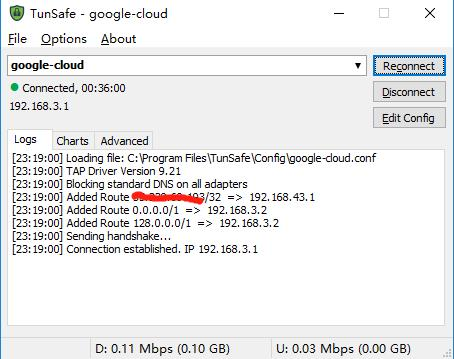
\includegraphics[scale=0.7]{wireguardtunsafeclient.jpg}
	\caption{Wireguard Windows客户端tunsafe}
	\label{fig:wireguardtunsafeclient}
\end{figure}

确保服务器开启了IPv4转发:

\begin{lstlisting}[language=Bash]
# 临时开启IPv4转发
sysctl net.ipv4.ip_forward=1
\end{lstlisting}

编辑 /etc/sysctl.conf 文件,查找到 net.ipv4.ip\_forward 这一行,改成 1开启转发,永久生效。iptables 里 filter 表的 FORWARD 链的 policy 是否为 ACCEPT。 nat 表的POSTROUTING链里是否已经做了出口的 NAT。如果还没有,使用以下命令加上:

\begin{lstlisting}[language=Bash]
iptables -t nat -A POSTROUTING -o eth0 -j MASQUERADE
\end{lstlisting}

在本地加上路由,把流量转发到 wg0 接口上:

\begin{lstlisting}[language=Bash]
ip route add <endpoint>/32 via <出口接口的网关IP> dev <出口接口>
ip route add 34.80.1.136 via 192.168.3.2 dev 192.168.3.1
ip route add default via 192.168.3.2 dev wireguard src 192.168.3.1
# 添加目标为 0.0.0.0,子网掩码为 0.0.0.0
# 下一个跃点地址为 192.168.43.26,跃点数为 7 的路由
route add 0.0.0.0 mask 0.0.0.0 192.168.43.26 metric 55
# 删除目标为 10.41.0.0,子网掩码为 255.255.0.0 的路由
route delete 0.0.0.0 mask 0.0.0.0
\end{lstlisting}

\subsection{应用}

利用Google Cloud公网IP搭建Wireguard后,可以形成一个虚拟的局域网,同时可以利用此环境做许多事情,当然任何事情首先得遵守相关规定。例如可以访问Google,查找资料、可以访问Google学术,搜寻全球的论文、自己搭建集群环境、自己编写应用部署到Google Cloud、访问局域网你们的设备、搭建自己的博客、申请自己的域名映射到Google Cloud博客服务器等等。有了Wireguard搭建的VPN服务,还可以增加Google Cloud云主机的安全性,对外只暴露特定端口即可,其他应用可以直接通过内网IP进行访问。

\subsubsection{ssh登录}

使用Wireguad连接后,Google Cloud上的云虚拟机与本地的节点相当于在同一个局域网,那么可以使用普通的SSH直接登录到Google Cloud远程虚拟机。更进一步,可以将连接上Wireguad的所有节点当成是一个本地局域网,不同的主机在不同的物理位置,这样就可以更加方便的搭建集群环境。虽然由于物理主机像个太远造成的网络延时无法应用于实际的生产,但是作为平时的学习研究还是可以接受的。

\begin{lstlisting}[language=Bash]
# 编辑sshd配置,允许root用户登录(不安全)
vim /etc/ssh/sshd_config
# 重新启动ssh守护进程
service sshd restart
# 利用内网IP登录到Google Cloud主机
ssh root@10.142.0.2
\end{lstlisting}




\newpage
~\vfill

\chapter{Docker}

\section{Docker基础}

\subsection{为什么要用Docker}

好不容易配置部署了redmine,结果后面换了一台机器,又重新部署一遍?其实绝大部都是配置的工作,繁琐又重复,其实我们没有办法也没有必要记住每一步操作步骤,先安装什么,安装好了再修改哪个文件的配置,重复的劳动没有任何意义。开发过程中会发现,许多工作都可以总结出来套路的,做过一遍之后,以后的内容都是高度重复。比如安装个软件,部署个应用,特别时多机部署,要保证一致性非常麻烦。还有经常会有的问题:在我的电脑上好好的呀?以上这些问题,就是Docker要解决的问题,可大量减少花费在维护、配置不同系统的时间。常用命令:

\begin{lstlisting}[language=Bash]
# 查看当前运行的容器
docker ps
# 登陆Docker容器
docker exec -it f5605d02f9f5 bash
# 登陆Docker后,登陆MariaDB
mysql -h127.0.0.1 -uroot -p123456
\end{lstlisting}


\subsection{Docker安装}

\subsection{安装数据层}

查看MariaDB:

\begin{lstlisting}[language=Bash]
docker search mariadb
\end{lstlisting}

安装MariaDB:

\begin{lstlisting}[language=Bash]
docker pull mariadb
\end{lstlisting}

安装时,从国外镜像下载的速非常非常慢,首先将下载源调整为国内的下载源。对于使用systemd的系统,在/etc/docker/daemon.json中写入如下内容(不存在此文件新建即可):

\begin{lstlisting}
{
	"registry-mirrors": [
		"https://registry.docker-cn.com"
	]
}
\end{lstlisting}

运行容器:

\begin{lstlisting}[language=Bash]
docker run --name MariaDB \
	-p 3306:3306 \
	-v /data/db/mariadb:/var/lib/mysql \
	-e MYSQL_ROOT_PASSWORD=123456 \
	-d mariadb
# 运行Jenkins
docker run -p 8080:8080 \ 
	-p 50000:50000 \ 
	-v /usr/local/work/jenkins:/var/jenkins_home \ 
	--name j01 -idt jenkins
\end{lstlisting}

p表示要自定义映射的端口(port),可以用-p hostPort:containerPort。为了方便迁移数据库中的数据,可以通过挂载数据卷(volum	e)来实现。这样,数据库中的数据将保存在我们挂载的本地文件/data/db/mariadb的上。我们可以迁移或者备份这个文件夹,来实现数据库迁移。一般一个自动生成的空数据库文件,大概有100多兆 ,而且这个文件夹中包含很多子文件,因此如果通过SSH或者FTP传输都需要比较长的时间,可以通过压缩打包来减少文件夹的容量。启动MariaDB镜像:

\begin{lstlisting}[language=Bash]
# 启动MariaDB
docker run --name mariadb -p 3306:3306 -e MYSQL_ROOT_PASSWORD=password -d mariadb

# 启动Jenkins
docker run -p 8080:8080 -v /usr/local/work/jenkins:/var/jenkins_home -t jenkins
\end{lstlisting}

启动Jenkins可能会出现如下错误:

\begin{lstlisting}[language=Bash]
touch: cannot touch ‘/var/jenkins_home/copy_reference_file.log’: Permission denied
Can not write to /var/jenkins_home/copy_reference_file.log. Wrong volume permissions?
\end{lstlisting}

当映射本地数据卷时,/home/docker/jenkins目录的拥有者为root用户,而容器中jenkins user的uid为1000。需要调整目录权限:

\begin{lstlisting}[language=Bash]
sudo chown -R 1000:1000 /home/docker/jenkins
\end{lstlisting}

启动后就可以通过本地的8080端口登陆Jenkin了。

\subsection{Docker导入导出}

查看名称:

\begin{lstlisting}[language=Bash]
docker ps
\end{lstlisting}

导出:

\begin{lstlisting}[language=Bash]
docker import -o MariaDB.tar MariaDB
\end{lstlisting}

导入:

\begin{lstlisting}[language=Bash]
docker export MariaDB.tar MariaDB
\end{lstlisting}

\part{Network}

\chapter{Web Service}

\section{Java Web Service}

再Intellij Idea中新建Axis Web Serive客户端时,Intellij Idea会在填入WSDL(网络服务描述语言,Web Services Description Language)链接后请求服务器,对链接做有效性检查。所以在创建客户端时,要保证Web Service服务端的联通,否则客户端会提示WSDL url is not valid。获取天气信息的测试地址\footnote{\url{:http://ws.webxml.com.cn/WebServices/WeatherWS.asmx?wsdl}}。

\chapter{HTTP}

\section{Fiddler}

\subsection{排查Google Api拒绝原因}

在抓取Google API数据的过程中,部署到部分机器上提示Connection was refused by other side: 111。原来是在本机调试的时候设置了代理,而部署到墙外服务器没有安装代理软件,其实根本不需要代理。去掉中间件(middleware)中的代理即可,移除如下代码片段:

\begin{lstlisting}[language=Python]
proxy_address = '127.0.0.1:8888'
request.meta["proxy"]="https://" + proxy_address
\end{lstlisting}

当然也有可能是服务端识别到了爬虫的请求头。在使用urllib库时,默认的请求头是:Python-urllib/3.7,很明显不是浏览器发出,服务器会认为是自动的robot发出此请求,无情予以封锁。Python发出的HTTP请求头可以在Fiddler中查看:

\begin{figure}[htbp]
	\centering
	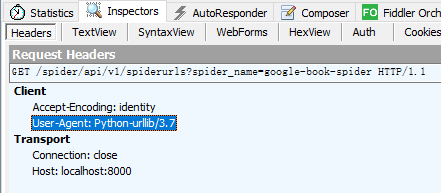
\includegraphics[scale=0.9]{fiddlercapturerequestheader.png}
	\caption{Fiddler查看Python HTTP请求头}
	\label{fig:fiddlercapturerequestheader}
\end{figure}

同样的,可以通过Fiddler查看请求Google API的请求头,从而通过调整请求头,避免被服务端识别。有的服务器会检查refer请求头,只允许本站的链接,从而避免外链,避免其他网站链接嵌入从而消耗自身的宝贵服务器资源。


\subsection{Fiddler与Shadowsocks冲突}

在安装了Fiddler后,浏览器直接通过Shadowsocks代理无法科学上网了。估计是流量无法经过HTTP代理层到Socket代理层。Socks 不要求应用程序遵循特定的操作系统平台,Socks 代理与应用层代理、 HTTP 层代理不同,Socks 代理只是简单地传递数据包,而不必关心是何种应用协议(比如FTP、HTTP和NNTP请求)。


\section{Web Server}

\subsection{CIDR(Classless Inter-Domain Routing)}

CIDR\footnote{\url{https://en.wikipedia.org/wiki/Classless_Inter-Domain_Routing}}(Classless Inter-Domain Routing)采用各种长度的"网络前缀"来代替分类地址中的网络号和子网号,其格式为:IP地址 = \{<网络前缀>,<主机号>\}。为了区分网络前缀,通常采用"斜线记法"(CIDR记法),即IP地址/网络前缀所占比特数。例如:192.168.24.0/22表示32位的地址中,前22位为网络前缀,后10(32-22=10)位代表主机号。在换算中,192.168.24.0/22 对应的二进制为:1100 0000(192),1010 1000(168),0001 10\textcolor{red}{00}(24),\textcolor{red}{0000 0000}(0)其中红色为主机号,总共有10位。当这10位全为0时,取最小地址192.168.24.0,当这10位全为1时,取最大地址192.168.27.255。本例中将第三段地址数据中最小是00011000(24),最大是00011011(27),第四段地址数据中最小为0000 0001(1),最大为1111 1110(254),以上括号中数据为十进制,其前面为二进制。所以本例中192.168.24.0/22 对应地址段为192.168.24.1-192.168.27.254,共4个网段。


\begin{table}[htbp]
	\caption{IPv4 CIDR}
	\label{table:ipv4cidr}
	\begin{center}
		\begin{tabular}{|c|c|c|p{3cm}|}
			\hline
			\multirow{1}{*}{地址格式}
			& \multicolumn{1}{c|}{网段}
			& \multicolumn{1}{c|}{子网掩码} 
			& \multicolumn{1}{c|}{主机数}\\			
			\cline{1-4}
			a.b.c.0/24 & +0.0.0.255 &  255.255.255.0  & 256 \\
			\hline							
		\end{tabular}	
	\end{center}
\end{table}

\subsection{maxPostSize}

maxPostSize=0表示post请求不限制大小,从 apache-tomcat-7.0.63开始,参数 maxPostSize 的含义改变: 如果将值设置为 0,表示 POST 最大值为 0,不限制 POST 大小需要将值设置为 -1。,在此版本之前设置为 0 表示不限制 POST 大小。The maximum size in bytes of the POST which will be handled by the container FORM URL parameter parsing. The limit can be disabled by setting this attribute to a value less than zero. If not specified, this attribute is set to 2097152 (2 megabytes)\footnote{\url{https://tomcat.apache.org/tomcat-8.0-doc/config/http.html}}.在7.0.63 版本之后要设置成小于0的数字才表示不受限制,另外此参数只适用于request的Content-Type为“application/x-www-form-urlencoded。排查此问题,可以在服务端查看接收到的消息体内容:

\begin{figure}[htbp]
	\centering
	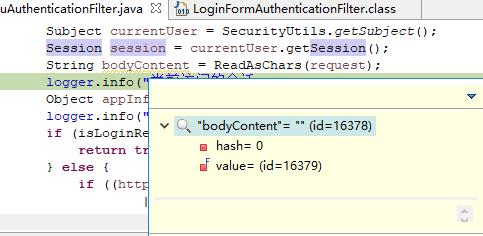
\includegraphics[scale=0.8]{loginrecievebody.jpg}
	\caption{登录接收到的消息体}
	\label{fig:loginrecievebody}
\end{figure}

从图\ref{fig:loginrecievebody}中可以看出,接收到的消息体为空,登录时用户名和密码放在消息体中,不可能为空,那么可以定位到由于服务端没有接收到请求的消息体导致程序问题。

\subsection{URL自动重定向}

在开启Fiddler代理的情况下(Fiddler代理端口8888),在浏览器中访问8082端口时,不管输入什么地址,都会重定向到一个网址。查看8888端口占用情况:

\begin{lstlisting}[language=Bash]
netstat -ano|findstr 8888
\end{lstlisting}

a(all)选项表示显示所有连接和侦听端口,n(number)表示以数字形式显示地址和端口号,o(own)选项表示显示拥有的与每个连接关联的进程 ID。发现有3个进程占用此端口(Chrome/Fiddler/Nginx),那么可以肯定是Nginx配置了自动跳转:

\begin{lstlisting}[language=Bash]
server {
    listen       8888;
    server_name  dolphin.spider.com;      

    location / {
        return 301 https://dolphin.spider.com:443$request_uri;
    }
}
\end{lstlisting}

将Nginx监听8888端口调整即可解决此问题。


\part{Book}

人类从古至今,总共有多少本书,答案是129,864,880\footnote{\url{http://booksearch.blogspot.com/2010/08/books-of-world-stand-up-and-be-counted.html}}。


\chapter{Paper}

\section{Font}

\subsection{类型}



\section{纸的种类}

\subsection{宣纸(Xuan Paper)}

宣纸又名泾县纸,出产于安徽省宣城泾县,以府治宣城为名,故称“宣纸”。宣纸是一种主要供中国毛笔书画以及装裱、拓片、水印等使用的高级艺术用纸张。宣纸拥有良好的润墨性、耐久性、不变形性以及抗虫性能,是中国纸的代表品种。宣纸起于唐代,历代相沿,由于宣纸有易于保存,经久不脆,不会褪色等特点,故有“纸寿千年”之誉\footnote{\url{https://zh.wikipedia.org/wiki/\%E5\%AE\%A3\%E7\%BA\%B8}}。

\subsection{连史纸}

\subsection{美浓和纸}

美浓和纸的历史起源于正仓院珍藏的户籍。据说薪火传承的手抄纸至今已经有约1300年之久的历史。只有纯手工制作才能展现的质感与出色特质至今依然丝毫不变。

%----------------------------------------------------------------------------------------
%	BIBLIOGRAPHY
%----------------------------------------------------------------------------------------

\chapter*{Bibliography}
\addcontentsline{toc}{chapter}{\textcolor{ocre}{Bibliography}}
\section*{Books}
\addcontentsline{toc}{section}{Books}
%\printbibliography[heading=bibempty,type=book]
\section*{Articles}
\addcontentsline{toc}{section}{Articles}
%\printbibliography[heading=bibempty,type=article]

%----------------------------------------------------------------------------------------
%	INDEX
%----------------------------------------------------------------------------------------

\cleardoublepage
\phantomsection
\setlength{\columnsep}{0.75cm}
\addcontentsline{toc}{chapter}{\textcolor{ocre}{Index}}
\printindex

%----------------------------------------------------------------------------------------

\end{document}


